% Modified
\documentclass{l3proj}
\usepackage{wrapfig}
\usepackage{csquotes}
\usepackage{glossaries}

\newglossaryentry{JQuery}
{
	name=JQuery,
	description={A free and open source JavaScript library that is used by Web developers to navigate HTML documents, handle events, perform animations and add \gls{AJAX} interactions to Web pages}
}
\newglossaryentry{HTML}
{
	name=HTML,
	description={HyperText Markup Language, the authoring language used to create documents on the World Wide Web.}
}
\newglossaryentry{CSS}
{
	name=CSS,
	description={Short for Cascading Style Sheets, a new feature being added to HTML that gives both Web site developers and users more control over how pages are displayed}
}
\newglossaryentry{Python}
{
	name=Python,
	description={An interpreted, object-oriented programming language developed by Guido van Rossum.}
}
\newglossaryentry{Javascript}
{
	name=JavaScript,
	description={A scripting language developed by Netscape to enable Web authors to design interactive sites.}
}
\newglossaryentry{Leaflet}
{
	name=Leaflet,
	description={A modern open-source JavaScript library for mobile-friendly interactive maps.}
}
\newglossaryentry{API}
{
	name=API,
	description={Application Program Interface, is a set of routines, protocols, and tools for building software applications. }
}
\newglossaryentry{Django}
{
	name=Django,
	description={A free and open source web application framework, written in Python, which follows the model–view–controller architectural pattern.}
}
\newglossaryentry{MySQL}
{
	name=MySQL,
	description={MySQL is an open source relational database management system that relies on SQL for processing the data in the database.}
}
\newglossaryentry{Git}
{
	name=Git,
	description={A distributed revision control and source code management system with an emphasis on speed.}
}
\newglossaryentry{PIP}
{
	name=PIP,
	description={A package management system used to install and manage software packages written in Python}
}
\newglossaryentry{Ubuntu}
{
	name=Ubuntu,
	description={A community-developed Linux-based operating system that can be used on desktops, laptops and servers.}
}
\newglossaryentry{W3C}
{
	name=W3C,
	description={World Wide Web Consortium, an international consortium of companies involved with the Internet and the Web.}
}
\newglossaryentry{AJAX}
{
	name=AJAX,
	description={Asynchronous JavaScript and XML, it is a term that describes a new approach to using a number of existing technologies together.}
}

\makeglossaries
\SetBlockEnvironment{quotation}
\begin{document}
\setcounter{secnumdepth}{3}
\title{Multi-device Recording System - MDRS}
\author{Alastair Weir \\
        Gordon Adam \\
        Peter Yordanov \\
        Keir Smith \\
        Georgi Dimitrov}
\date{28 March 2014}
\maketitle
\begin{abstract}

Surrounding us in city life there are unique moments missed everyday by experiencing  them through the lens of a smartphone instead of being 'in the moment'. That instance is lost in time and never fully appreciated. The video or images captured are then restricted to that specific person, only able to relive the moment from their limited perspective. By creating a mobile first approach to capturing locational audio centred around these moments, MDRS can offer new insights and crowdsource distinctive, new  perspectives of life in our cities. This aim was successfully achieved with a functioning web and mobile application to allow users to gather this information while still enjoying the moment, then later explore their perspective and others in a unique way. Our testing has shown...

\end{abstract}
\educationalconsent
\tableofcontents
%==============================================================================
\chapter{Introduction}
\label{intro}

\section{Motivations}
Around the world, ubiquitous connectivity is giving users a new avenue to make their voices heard and share their stories. With MDRS (multiple device recording system) we leverage a mobile device’s sensors and give everyone a platform on which share their story, or experience, in a specific place and time. These all join to form a map where others can explore and listen to these experiences synchronously in chronological order. If more than one recording happens in the same area at the same time they will playback together, melding to create an unique and richer insight into an event such as a concert.

In recent years concert attendees have derided a rising trend of viewing an amazing live performance, happening mere metres away, through a sea of smartphone screens in front of them. These screens detract from an attendee's enjoyment to the extent that  some bands ask their fans to not use their phones during their performance. MDRS is a step beyond this frustration as it's passive, letting a user record clips of the concert to share with their friends later while their phone is still in their pocket. This frees their attention to immerse themselves in what is happening. Users can actively improve the experience of the concert for everyone while still creating something they can share with friends later.

In the case of a festival, bands could upload their own recording of their performances with professionally captured images and the location of their stage within a festival site. These uploads could create a concentrated virtual space populated with dozens of  professional recordings and the crowd’s experiences for users to explore and gain a noteworthy perspective they might have missed at the time.

MDRS could also be used in law enforcement and political movements. It's unique storytelling ability to combine the spoken word and images while communicating an accurate sense of place sets it apart from alternative methods. By giving an investigator multiple perspectives to an incident, they can ensure that a fair judgement is passed. If a victim is struggling to find justice they can effectively ‘crowd-source’ their evidence from those who are present. This would help to keep political protesters safe and protect their rights when dealing with law enforcement. MDRS gives a voice to unheard or mistreated minorities.

These use cases are a slice into the motivation that drives this innovative project. They demonstrate a rare opportunity to leverage some of the vast data our smart devices are capable of capturing from the physical space and generate something original.

\section{Aims}
As more connected mobile devices reach the hands of consumers, billions of pieces of data are being created every day. A lot of this data is based around events in people’s lives from large scale political movements such as the Arab Spring to a friend's birthday party. Extracting meaning from these colossal stores of data created by this internet of things is one of the key challenges in technology today.

MDRS aims to allow people to easily share important experiences and moments through a combination of location, audio recordings and images. We aim to leverage Android as the dominant mobile platform around the world. This offers a large install base with many possible uses for MDRS instead of catering for a narrower user type. The app should be able to passively record in the background allowing its user to actively participate in the event happening around them. This removes the conscious decision to become a passive documenter instead of participating in what is happening.

A web application will allow users to explore the recordings uploaded in an interactive map. They will be able to search for specific events or select all recordings in an area for synchronous playback. By achieving this unique playback style accurately synchronised in time, MDRS offers a more meaningful way to explore data than listening to recordings individually. We aim to surprise and inform our users by offering them insights into different cultures, walks of life or new perspectives on events in their own lives. We believe the service should be free to use and access, offering a simple and attractive interface across it's two platforms.

\section{Background}
Mobile was an interest in many of the team members and a trending sector in the technology industry. These devices have surpassed the use of computers in the home and are of particular interest to User Interface/User Experience designers. Their screen sizes, use cases and interaction models are very different to traditional devices and developers are constantly finding new innovations in this field. With the proliferation of wearable devices such as smartwatches with arrays of sensors embedded, finding new use cases are an area of interest.  Android’s support for varied screen sizes and device types gives the team a welcome technical challenge while making use of our existing knowledge of Java.

Designing for the web incorporates numerous disciplines and a good foundation in a number of syntaxes. This makes for a steep learning curve but by leveraging previous experience and through other coursework undertaken throughout the year, acquisition of the required skills becomes much easier. To build a lightweight web client means leveraging core web technologies such as \gls{HTML} and \gls{CSS} to their fullest to improve the user’s experience as much as possible while keeping the application lean and fast. Where needed \gls{Javascript} is used to add more dynamic features desired to the project.

Deploying a web application can be done in many different ways with innumerable frameworks and tools available to use. Again, hoping to use pre-existing skills we researched and hoped to use a \gls{Python} based framework as the basis for MDRS’ backend.  The language's versatility made it an ideal choice while not adding to the heavy workload the project demanded with another new language to learn.

Today in the market, very few systems similar to MDRS can be found for use. Services such as Soundcloud or Audioboo allow the user to easily record audio and upload it to a website for sharing but beyond that offer limited functionality. These both heavily focus on the social interaction around each recording. Software such as Audacity would allow the user to manually stitch the audio together but this process is technical and time consuming.

The only product that matches more of MDRS’ aims is Broadcastr. A New York City based startup now renamed SPUN released Broadcastr in 2010, allowing users to record stories and link them to a static location. The app gained media attention upon release with recommendations from the BBC and Wired. SPUN later abandoned the project and moved into geo-targeted advertising. While similar, Broadcastr still differs as MDRS allows for a recording to forge a path across the map, linking the audio and images to a user’s location as they move through a place. This project takes the best from its competitors and adds new layers of functionality, offering more, in the hope of making something truly worthwhile.

\section{Preliminaries}
To fully understand this dissertation, the following knowledege would be beneficial:
\begin{itemize}
\item A basic understanding of the construction of an Android application
\item A basic understanding of how \gls{Django} projects function
\item Syntactic understanding of Java, Javascript and Python
\item Willingness to follow the links to the various resources used as part of MDRS
\end{itemize}

%==============================================================================
\chapter{Research}
\label{Research}

The first step in conducting our research was to research pre-existing applications both on mobile and the web. We investigated applications that were already established on the market with similar features in order to learn what had been proven not to work and new areas of untapped potential.

\subsection{Soundcloud}
Soundcloud according to its website is:
\blockquote{An audio platform that enables sound creators to upload, record, promote and share their originally-created sounds.}
This website offers an excellent way for users to share their music and sounds with others and for these users to comment on their favourite part of the upload, linking their message to a timestamp. Soundcloud's main attraction is this social interaction fans can have with content creatiors. However the majority of people uploading on this website are artists uploading their music. In MDRS we aspire for everyone to be able to upload the recordings they take in many different situations.

\subsection{Audacity}

On the desktop there are a number of applications that allow you to manipulate audio and combine multiple files. Audacity is a popular desktop application that allows the user to record and convert audio. It also allows the user to cut, copy and splice together recordings. The ability to merge audio files together was a key requirement of MDRS that the team needed to implement. However our application would need it done dynamically "on the fly" to allow the user to quickly change which audio files were played back together. In order to accomplish this task in Audacity is too slow and technical for a typical user.

\subsection{Foursquare}

Foursquare is a location based mobile app that the group found to incorporated much of the functionality we desired in our project. It allows users to "check in" at certain locations and add comments or pictures about a place or event. There is also a web application allowing other users to see the most recent data in their area very easily. However this is as far as Foursquare goes, with no ability to share audio. The ability to playback audio synchronously with nearby surrounding recordings will completely change the user's experience offering a far more immersive insight into a user's surroundings.

\begin{figure}[ht!]
  \centering
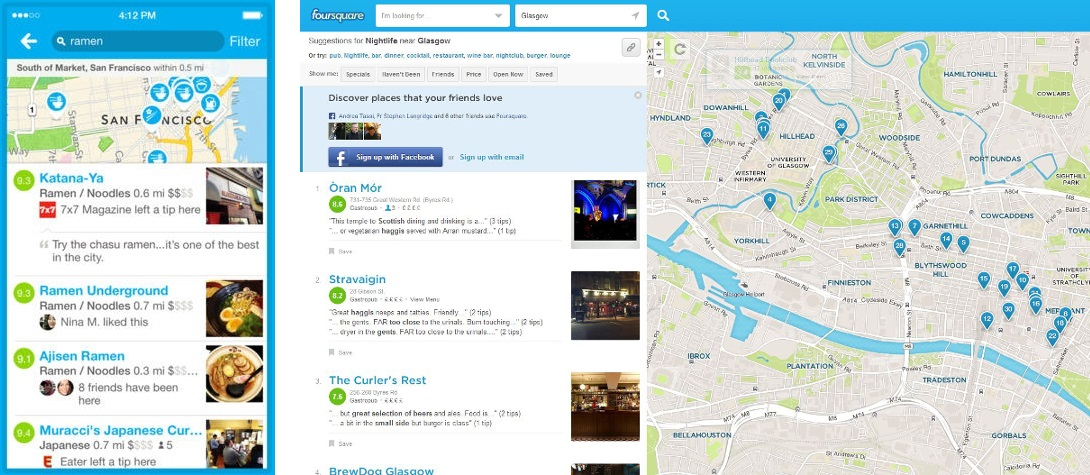
\includegraphics[width=0.75\textwidth]{images/foursquare.jpg}
\caption{Foursquare Mobile App (left) Foursquare Web App (right)}
\end{figure}

\section{Initial Research Conclusions}

After this it was decided to split the project into two separate parts, discrete web and mobile applications. This direction was chosen from the research carried out. Foursquare had a strong influence over the decision. It was found that the end users experience can be greatly enhanced with the inclusion of a web application to accompany the mobile side. This would also allow a greater number of features to be incorporated into the project. If the project had been purely mobile the limitations of the platform could lead to a poor user experience with a cluttered and confusing interface, limiting the usefulness of MDRS.

The team acknowledged this dual aim would also help distribute the work amongst themselves. On the other hand it was recognised that a greater amount of work would be taken on by the group to complete these two applications. However, everyone was enthusiastic about making this extra effort in order to make a more rounded and complete final product.

For recordings taken by the mobile application to be represented as clearly as possible on the web application we consulted as a group as well as with our project supervisor, it was decided that each recording would have to be represented in both time and space. To do this as effectively, it was agreed visual aids would be the clearest way to represent this information. So the use of a map view was decided to represent the recordings spatially and a timeline to represent them chronologically.

\section{Web Technologies}

With the potential MDRS possessed, realised, it was essential for the team to research key features and tools that we hoped to integrate into the project and to find things that would fit well into our imagined product. This enhanced the team's collective knowledge on a battery of topics and tools greatly, allowing us to make the right decisions for the project.

\subsection{Map}

OpenStreetMap was initially the preferred choice of mapping data. Deep open source roots combined with an excellent level of detail and accuracy was attractive. When combined with the Javascript library \gls{Leaflet} to embed the map, the potential was excellent. OpenStreetMap's downfall lay the need to store the raw map data, which uncompressed could comprise up to 400GB. Storing this on our server would be an impossibility. Some commecial options were available such as MapBox which host this data but these services offered very little in their free products. And while Leaflet would support our central aims, its limited functionality restricted the possible direction the team could take MDRS in. The default style for OpenStreetMap was also far more detailed, reducing readability and cluttering an interface we aimed to keep simple.

\begin{figure}[ht!]
  \centering
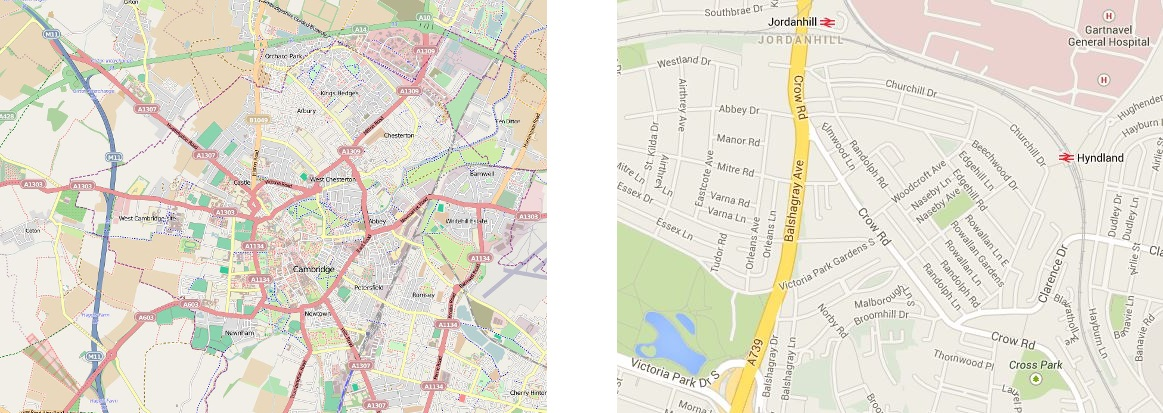
\includegraphics[width=0.75\textwidth]{images/openstreetmap_google-map.jpg}
\caption{OpenStreetMap (left) Google Map (right)}
\end{figure}

Google Maps was seen as a strong alternative. While it was not open source, it offered comparative quality of mapping data. A weakness was found in the limitations set on the free use of the \gls{API}. It was found that after the obtaining of an API key however we would have access to 25,000 user visits a month.\footnote{This number of visits was derived by taking the number of map loads offered to free users of Google's API and dividing it by the number of map views estimated for each user's visit to MDRS} It was decided this limitation would not affect MDRS in its early stages. The default map style for Google Maps was far more simplistic  fitting more neatly with our designs. The API documentation for Google Maps was also excellent giving many examples and walkthroughs which would help make development considerably less confusing.

Taking these points into account it was decided that we would use Google Maps as no extraneous data would be stored on our server and the API appeared to be easier to use.

\subsection{Timeline}

%The use of a timeline of recordings was central to MDRS' iteration conceit. TimelineJS offered an attractive UI populated with clear boxes for each event that when clicked on, centred the timeline to that element and associated metadata would be displayed above it. It was found to be effective in clearly communicating the difference between recordings, portraying a vertical line on the timeline for each event. The metadata view above the timline, while unnecessary for the front page, would be crucial for the user's profile view. Importantly for MDRS, this timeline is also well supported on mobile devices.

%\begin{figure}[ht!]
%  \centering
%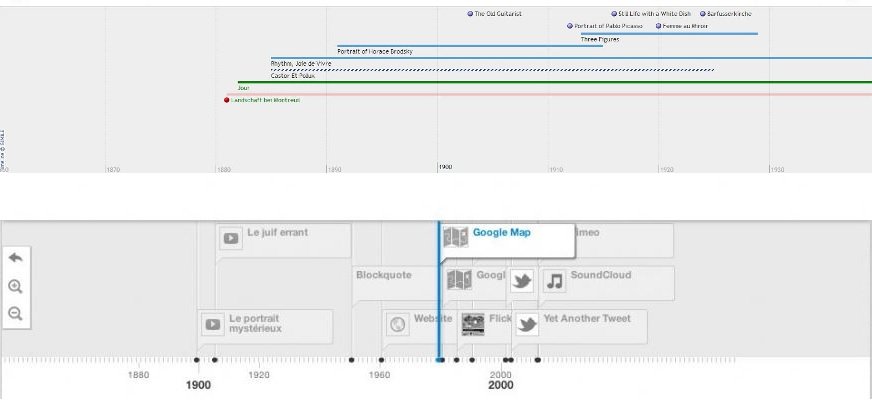
\includegraphics[width=0.75\textwidth]{images/similie_knightlab_timeline.jpg}
%\caption{MIT's SIMILIE Timeline (top) Knightlab's Timeline JS (bottom)}
%\end{figure}

%Another timeline that was researched was the SIMILIE Timeline, developed by MIT. The main point of contention with this timeline is in it's appearance, which falls much further short of it's contenders. There was also some questions about it's compatibility with Internet Explorer and mobile devices. The upside however is that it offers a greater level of customisation, allowing much more flexibility with it's styling.

%After a comparison TimelineJS was chosen due to its ease of use for the end user and its attractive user interface which was deemed a more important feature than greater customisability. Also the compatibility issues of the SIMILIE timeline could have caused problems further down the line, which we may not have been able to resolve.

In order to display the recording information in an informative format, we identified a timeline presenting the recording objects in linear time as a key requirement for MDRS. This would give the team the opportunity to implement a user-friendly interface, enabling the user to easily identify overlapping recordings in the database. Ideally the timeline would display,

\begin{itemize}
\item{Recording's title}
\item{A recording's duration}
\item{A recording's start time}
\item{A recording's end time}
\end{itemize}

When clicked on, the following information would be revealed to the user:
\begin{itemize}
\item{The uploader}
\item{A recording's description}
\item{Accompanying imagery uploaded by the user}
\end{itemize}

After having clearly specified, documented and researched the functional requirements in order to try and find the best way to implement this key component for the system, we made design decisions and integrated it in the system. Having tested a number of different open source Javascript implementations of different timelines, the final decision was based on the implementation differences and the degree of customization those products offered (all implemented in JavaScript):


- \textbf{SIMILE timeline} - http://www.simile-widgets.org/timeline/

- \textbf{Timeline JS} - http://timeline.knightlab.com/ (GitHub repository - https://github.com/NUKnightLab/TimelineJS)

- \textbf{Chronoline} - http://stoicloofah.github.io/chronoline.js/

- \textbf{TimeGlider} - https://github.com/timeglider/jquery_widget (moved here a year ago: http://timeglider.com/widget/)

- \textbf{Chaps Timeline} - http://almende.github.io/chap-links-library/timeline.html



\textbf{SIMILE}

\begin{figure}[ht!]
  \centering
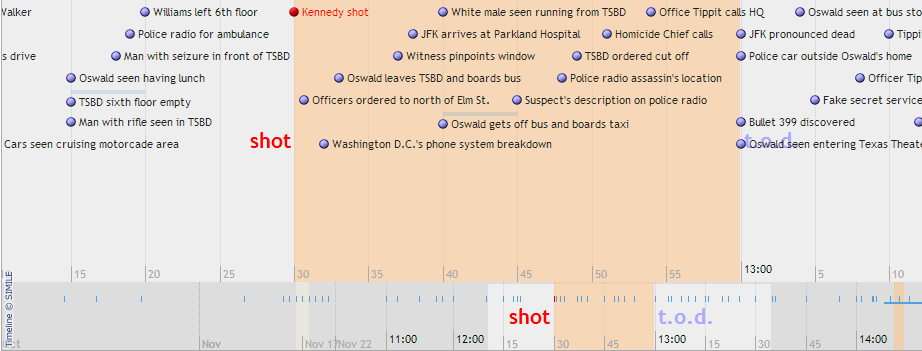
\includegraphics[width=0.75\textwidth]{images/SIMILE.png}
\caption{SIMILE timeline}
\end{figure}

The SIMILE timeline (this product is implemented in javascript), is a very good example of an efficient and compact timebar able to accommodate a number of events in a relatively small space without looking too clustered with unnecessary information. It also supports scrolldown horizontal movement and  you can click and drag to navigate between objects using your mouse. However, there are a number of drawbacks associated with this open source implementation. To start with, its maintainability is poor - the last change that was made to the source code was in May 2009 which is very very long ago. We also researched the opinions of people who have tested it online and found out that there are mixed feelings regarding the SIMILE timebar. One of the issues people had experienced was memory leaks that were caused especially when dynamically loading and unloading events to the timeline. The poor maintenance of this product also had caused numerous people troubles with the implementation in different browsers as apparently there are many unidentified bugs that continue to increase with each browser update. Some people even had strange experiences of browser crashing as a result of using SIMILE (more information can be seen in this StackOverflow topic: http://stackoverflow.com/questions/4700419/alternative-to-simile-timeline-for-timeline-visualization). Customisation and updates are also very difficult considering the relative lack of documentation or poorly documented code segments which was also one of the main reasons why we decided that it will not be the most suitable option for what the user interface requires.


\textbf{Chronoline}

\begin{figure}[ht!]
  \centering
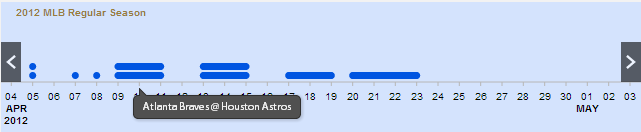
\includegraphics[width=0.75\textwidth]{images/Chronoline.png}
\caption{Chronoline timeline}
\end{figure}

The Chronoline timeline was also a very attractive alternative and it is really compact indeed. However, for the purposes of the multi-device recording system, it looked too simplistic and did not provide enough options for further customization in order to make it work as we would require. It also does not support mouse dragging when switching between the recording objects. After a thorough research we discovered a number of people that were having issues with this timeline as well and, although it is indeed a well maintained project, its documentation is poor.


\textbf{Timeglider JS}

\begin{figure}[ht!]
  \centering
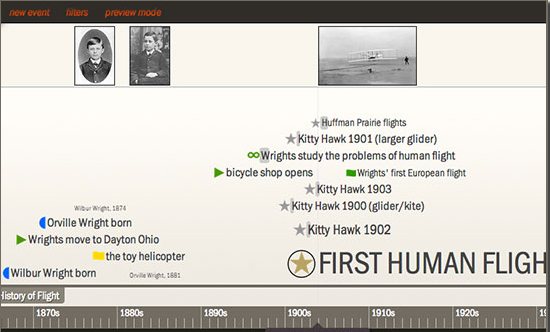
\includegraphics[width=0.75\textwidth]{images/Timeglider.png}
\caption{Timeglider timeline}
\end{figure}

Timeglider JS was an option which really captured the attention and took some time to test in order to see whether it would be a good option. It supports many features and has a number of sub-components however they were making it a little bit too complicated for what we actually needed and it looked kind of too demanding for the average user as it required some time to get used to and understand how to interact with it. This product is clearly documented, containing detailed information on how to use the API to customize it on the website which was created about a year ago when the code from the GitHub repository was transferred to timeglider.com. After carefully considering this option, we decided to continue searching before making a final decision.


\textbf{Chaps}

\begin{figure}[ht!]
  \centering
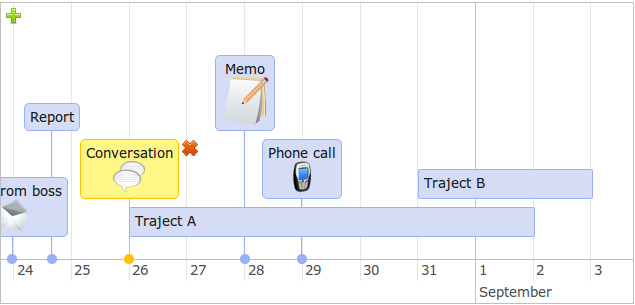
\includegraphics[width=0.75\textwidth]{images/Chaps.png}
\caption{Chaps timeline}
\end{figure}

The Chaps timeline, is also really impressive - not very heavy and at the same time, not too simplistic for what we needed. It supports mouse scrolling for zoom-in / zoom-out and mouse dragging in order to slide it horizontally as most of the other alternatives. It was also one of the viable options which we left to the side before making our final decision. However, when considering it, we noted a not very serious, but still significant drawback, which was easily fixable - it does not look very elegant and is not very dynamic, not allowing the user to switch between the object using left and right horizontal arrows. In addition, its structure would not suit very well with the rest of the user interface.


\textbf{KnightLab Timeline JS}

\begin{figure}[ht!]
  \centering
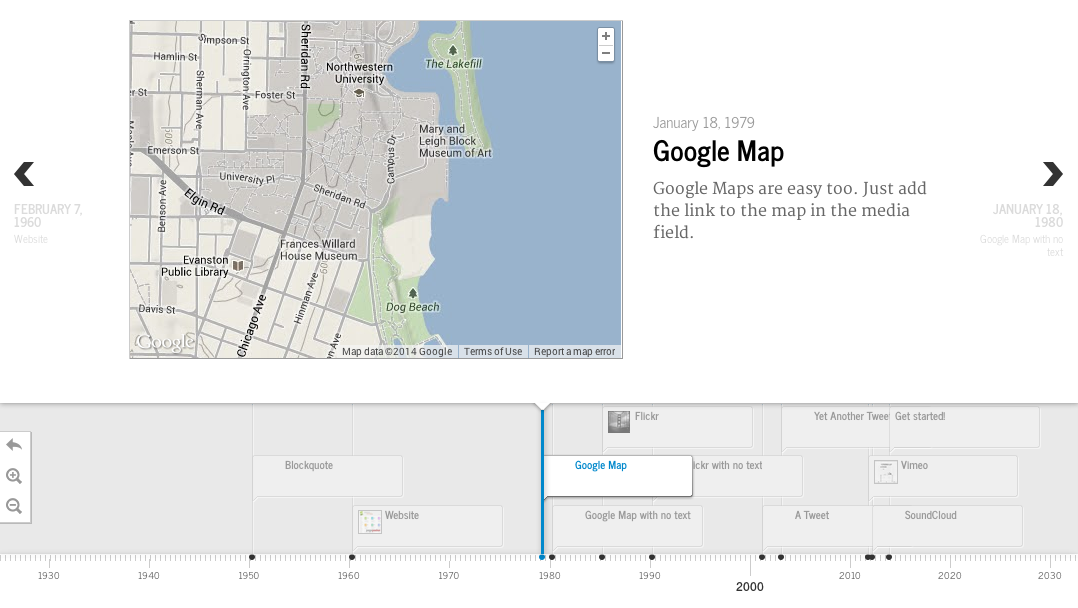
\includegraphics[width=0.75\textwidth]{images/timeline-example.png}
\caption{Knightlab Timeline JS}
\end{figure}

Last but not least important candidate - Timeline JS. This product is well maintained and has an active community contributing to its GitHub repository (https://github.com/NUKnightLab/TimelineJS), making it very user friendly and easy to test. It looked like a really flexible and customisable solution right from the start, but this needed to be verified after testing the product's functions. Timeline JS is coded in Javascript, CSS for styling and some python is used too.

One thing which really distinguishes it from the rest of the candidates is the fact that it is thoroughly documented in the repository as well as the website. And everyone is welcome to ask questions on their community forum, make changes or suggest some alterations to the code in the GitHub repository by opening new tickets for enhancements or bug fixing. We had some questions for the JSON template as we intended to use this format to dynamically feed the timeline with information extracted from the database and contacted their team. They responded quickly and gave us all the answers we needed (community forum: https://knightlab.zendesk.com/forums/22551396-TimelineJS) so this proves how well maintained this open source software is and made it even more attractive. It also provides simple and easy interaction when used from a mobile device such as a smartphone or a tablet, or any other touch-screen device.

Timeline JS also provides a number of customization options which are clearly documented on the website and it has a nice display field for which could be using for the recordings' metadata. The interface is extremely responsive and provides an elegant way of switching between recordings' information either by clicking a recording object or by using the provided left and right arrows for horizontal sliding. What is more, it has a bookmark built-in function which allows for recording object to be easily linked by using the format - #number - a hash tag followed by the recording id which would definitely prove useful at a later implementation phase. On top of that, we thought that being able to specify the exact starting point for the objects on the timeline was another huge benefit.

After comparing timeline JS with the other viable options and having contacted their representatives or making research on other people's opinions all over the internet, we were ready to make the final decision of the implementation to use. The fact that many developers, who were looking for an elegant and easy to customize, well documented, and clearly structured open source project easy to feed with dynamically generated JSON, after trying various different options, had discovered that Knight Lab’s Timeline JS works best for them, made us confident that choosing it would be the right thing to do. And so we did.



\subsection{Front-End Web Framework}

PureCSS is described on its website as,

\blockquote{“A set of small, responsive CSS modules that you can use in every web project.”}

This was an ideal candidate for our front-end framework as it was minimalistic in both size\footnote{PureCSS is 4.5KB when minified.} and appearance. The documentation for PureCSS was also extensive which would  ease problems the development process of a reactive front end.

Twitter's Bootstrap framework appeared to be a more complete solution. It provides icons, styling, and a number of UI elements ready to be easily added to a webpage. However in being the complete package, less flexibility would be offered in the appearance and the front end could end up having very little of it's own character. Performance also suffers due to the size of the Javascript and CSS files required.

Although Bootstrap had many more features, the majority of these were unnecessary for our project. Its inclusion would have needlessly complicated the web application whereas PureCSS gave a solid foundation to build our website upon. Its lightweight approach aligned and met our simple requirements


\subsection{Audio Playback}

'Buzz!' is a JavaScript library that utilises the HTML5 audio element. Again touted as a lightweight implementation, this library excelled grouping multiple audio files together and playing them simultaneously. It worked in the background requiring no user interface unless one was required of it. When implemented these could be simple HTML Buttons with Javascript commands attached to them. This offered the team a lot of control over the styling their audio playback.

JPlayer was also considered though it had drawbacks in playing multiple files as there appeared to be no obvious way to play multiple files without having multiple instances of the player UI. This had the potential to negatively impact performance in a big way. The JPlayer's unattractive, heavy UI would also have to be repeatedly used within our interface cluttering the design.

The team took the decision to use the 'Buzz!' JavaScript library as it was exactly what we were looking for on this particular occasion.

%==============================================================================
\chapter{Planning}
\label{Planning}

\section{Team Structure}This section will outline the organisational methodology used by the team during the lifespan of the project. This includes: the roles of each team member as well as their responsibilities, how is authority distributed amongst members, a conflict resolution strategy, communication and information management within the team, any identified risks involving the organisational approach chosen and the organisational model itself.

\subsection{Roles}After discussion, we have decided to use agile development, specifically scrums, to build our system. As part of this technique we need both a scrum master and a client representative, these roles will be outlined below. We chose this model considering a combination of different factors that influenced our final decision. For instance, the relatively small size of our team - there are five of us. Also, we needed to carry out rapid iteration cycles in order to meet the assignment delivery deadlines.

{\bf Scrum Master (Keir Smith)} - The scrum master will organise times and locations for the team to meet every week then chair the meeting, talking about progress and future development. The scrum master will also assign jobs and roles to developers as the project progresses and oversee their completion. In case we have some kind of a disagreement between the group members, the scrum master will mediate the situation and find a solution.

{\bf Client Representative (Gordon Adam)} - The main communicator with our project supervisor. He must remain impartial to the project and view it with the same mind set as the client would. The client representative will also be responsible for organisation of testers.

{\bf Developers (Alastair Weir, Petar Yordanov, Georgi Dimitrov)} - Despite the use of agile organisation there are still many traditional roles in software development such as Librarian, GUI designer and Architect.  These roles will be filled on an ad-hoc basis when and where needed and on people’s interest. We will not set them in stone.

All team members will be developers working on the different facets of our wide ranging project. Some members may take preference to certain areas of the project but ultimately it is down to the scrum master, after consultation, to what each member will be working on at any one time.

\subsection{Authority}Decisions in the group will be based on a democratic structure. Decisions shall firstly be discussed between the team members, either face to face or via one of our stated methods of communication. If we have a case where all team members agree on a given solution during discussion, there will be no need for a vote or further discussion.

If there is however a conflict between three or more members, the scrum master is to take control and a vote shall be cast and/or further discussion shall be held and led by the scrum master until a decision is made.

In case the conflict cannot be resolved by the steps taken as described above, we are going to contact (schedule a meeting for instance) our project supervisor and ask him to assist us in the resolution process.

\subsection{Communication}From the outset our group was keen to leverage the use of the third year lab space and regularly meet face to face. As we all have the same timetable and everyone is in the habit of spending time at the lab, we intend on having regular interactions to communicate issues. We we will also make use of the common room in the Sir Alwyn Williams building as it is not as busy as the lab. At minimum we will hold one formal meeting each week. Of course, asynchronous communication is also essential. We quickly set up a Facebook group within which we can post key information and decide on meeting times and share articles or documents that relate to our project. This was chosen as it is accessible from all platforms. To foster a greater sense of camaraderie, a group IM chat has been set up for unimportant communication and general chat.

All communication amongst the team will be transparent and visible to all. The tools we have selected will hopefully facilitate this successfully.

\subsection{Information Management}Our prefered methods of communication all keep logs of our conversations which allows us to review why we made decisions. In face to face meetings a secretary will take notes, so we can review our meetings and record how we have progressed through the development cycle.

For more indepth organisation we have set up a Redmine instance; this will allow us to keep track of our project, keep up with issues, track bugs, keep a wiki and assign roles/jobs. This is the project management system where we are going to record minutes of meetings as well as important discussions and decision.

We have decided to use \gls{Git} for version control as it’s a fantastic, free platform for multiple concurrent users working on a single project. We can also track this Git project via Redmine and keep the whole team up to date.

Also available is a shared team Dropbox for backup purposes. We will also use Google Drive’s collaborative documents feature when working on our dissertation and other hand-ins.

\subsection{Organisational Risks}The major identified risk is if one of our team members leaves or falls ill. Our agile team structure will hopefully manage to sidestep this danger. Another consideration we will take to prevent this issue is make sure more than one person is involved in each perceived division in the project. At the beginning of the project we have identified numerous sections: mobile, web, backend. By spreading the work amongst us we will avoid this danger.

There is also the possibility of a new team member being assigned a slot in our team. In such a case we are going to need to bring them up to speed with a training session which cannot be specifically limited in time as it depends on how far in the development process we have managed to get.

Other issues could be integrating new team members, data loss, an ineffective scrum master or client representative. In case the we find that the current master or our client representative are ineffective, we might organise a team meeting, vote and accordingly make changes if needed. We are going to organise sessions at the end of each sprint in order to gather feedback on performance - which targets have been met and whether or not the scrum master/ client rep./ developers have carried out their tasks as expected.

\section{Use Cases}
Continuing our preparations before implementation, the team considered and documented the possible use cases of the system in the form of paper-drawn storyboards. These blossomed into situations that MDRS could actively improve a user's experience giving us a grounding from which to work from.

<paper user stories images>

\subsection{Recording at a Demonstration} The synchronisation of multiple audio streams at a protest or any other type of public demonstration would enable the listener to hear different perspectives of the demonstration. What is more, they could switch between the source audio streams in order to distinguish speech, conversations, etc.

\textbf{Scenario:} John is a lecturer at a public protest in Glasgow regarding the academic salaries in the UK. He is at the protest with a couple of colleagues - Jane and Chris. However, the protest has not managed to attract that many people to support their cause

The three friends are trying to spread their message further by installing MDRS on their Android devices and recording conversations while at the protest. Then sharing the different views people express in their statements from multiple vantage points at the protest can be listened to by their fellow colleagues and opponents in the hope of making them understand their point of view better.

\subsection{Music Festival} Being able to synchronise multiple recordings from a music festival is also a possible use case for this application. It will give musiclovers who missed an event the opportunity to listen to it as if they attended, listening to the various vantage points used for the recordings. Also, noisy audio streams can be switched off to improve the audio quality of the playback.

\textbf{Scenario:} There is a music festival on a stadium in London and Tom (from Aberdeen) and Kate (from London), who know each other, have bought tickets and are going to attend the festival. However, they are not going together and do not know that are both going to be attending. Tom has a ticket for the front rows because he has been expecting to see his favourite band live for months, while Kate is there just for fun and has grabbed herself a cheaper ticket somewhere in the back.

They are both recording the event using the MDRS mobile app to upload it to their personal timeline later.

After the event, the pair meet each other by accident and talk to each other about how they are getting on with their lives. After uploading the recordings they made on the festival online, with the MDRS web application they will be able to compare switch between the audio streams and listen to both of them at the same time - the louder and clearer recording Tom made and the more noisy one Kate recorded. They would also be able to share their perspectives, Tom in the chaotic front and Kate with a great overview of the whole event unfolding.

\subsection{Home Party Recording} The multi-device recording system can also be used for other entertainment purposes, such as recording conversations from different locations at a house party. synchronised playback ofthe audio will be great fun to listen to on the next day after the party.

\textbf{Scenario:} David is hosting a house party and everyone starts recording people's conversations with their mobile devices scattered around in the rooms.

The next day after the fun is over, it is going to be greatly entertaining to listen to all the gossip people have been discussing.

\subsection{Sports Event} If there is a sports event such as a championship or a tournament which involves matches being played on numerous locations at the same time, it would be nice to be able to record commentators discussing the game and synchronizing their statements to keep track of the present result.

\textbf{Scenario:} Mark is a great fan of tennis and is attending a tennis tournament in France. He idolises Rafael Nadal and has bought tickets for his tennis match against Novak Djokovic, court 1. At the same time, however, on court 4 plays Roger Federer against Grigor Dimitrov.

Mark is a very keen supporter of the Bulgarian rising star but cannot be at that court at the same time. By using MDRS to record the match on court 4, one of Mark's friends who is also attending the tournament but has a ticket for the other section is able to deliver Mark the audio stream from the other tennis court, making it possible for mark to listen to judges on both courts to keep track of the result.

\section{MoSCoW requirements}
Listed below are the project functional requirements the team identified with their priority rating based on the MoSCoW system:

\subsection{Must Have}
	\boldit{Web application:} The system needs a website with a backend support for audio processing.

	\boldit{Mobile application:} Android application for audio capture to be submitted to the database of the website via an upload form.

	\boldit{User Authentication:} Potential users need to be able to register on the web application in order to keep track of each person's individual audio recordings and visited locations.

	\boldit{Recording audio:} The system mobile application needs audio recording functionality so that the user could quickly capture audio with the click of a button.

	\boldit{Recording submission:} Interaction between the Android app and the web application.

	\boldit{Storing audio recordings:} The mobile app needs to store recordings on the server for processing.

	\boldit{Audio synchronisation:} Audio synchronization functionality on recording selection.

	\boldit{Recording timeline:} A timeline to show database recordings based on their start and end time (as well as provide a temporal visualisation of overlapping recordings).

	\boldit{Map view:} Visualisation of each recordings position on a map view for a user to spacially explore.

\subsection{Should Have}
	\boldit{Playback selection:} Users need to be able to listen to all the recordings and be able to select.

	\boldit{HTML5 GeoLocation:} The web application should be able to find a user's current location and centre the map on this, revealling recordings in the local vicinity.

\subsection{Could Have}
	\boldit{Route tracking:} Once a user has started recording, the system needs to use GPS tracking to update current location and save it to the database when recording activity has finished.

	\boldit{Taking photos:} The Android application needs to enable the user to take photos while recording to enrich the playback experience.

	\boldit{Filter recordings by time and date:} Provide users the option to filter recordings and display only those from a specific time period on the map and the timeline.

\subsection{Would Have}
	\boldit{User account enhancements:} Offer enhanced user pages, friends list support and more social connections to other networks (Facebook, Twitter).

	\boldit{Recording grouping in events:} Allow users to create events and link their recordings to this, facilitating the retrieval of all recordings for a single event for other users.

	\boldit{Descriptive Tags:} Users could add relevant tags to their recordings which will enable easy search and recording filtering.


\section{Project Timeline}		From the outset, the team laid out a flexible timetable for the project, accounting for the series of phases a project must undergo.

During week one we filled the consent forms which were distributed to us after the group allocations were announced and submitted the ballot.

We had a couple of days to make a final decision on the final six projects from all the project proposals and created a Facebook page to help with the communication between group members in general and more specifically, as a form for project management beside the RedMine project management system we decided to use as a primary one.
After we understood the team project allocation, we started researching and planning about the key functional requirements how we are going to implement them, consulting the project supervisor on how to approach each design and implementation phase.

Having organised a couple of team meetings, we exchanged contact information and made a final decision on the system for version control and project management - Github and RedMine accordingly. Following a quick discussion we also took the decision to use the agile framework for the team structure and chose Keir as our scrum master. Most of us did not have experience using project management and version control software at first so we needed some time to learn the basics and get used to it. The more experienced team members helped those who had issues and gave advice in order to resolve contribution conflicts with the version control system.

During this period we also made important communication decisions. The team decided to meet face-to-face at least a couple of times on a weekly basis right before the supervisor meeting which we chose to be on Tuesday at 4 pm. in the afternoon. This team meeting we would use to discuss progress made during the previous week, analyze the targets met and potential experienced issues, as well as introduce new goals and tasks for the forthcoming week. Regarding virtual communication, we had a discussion about what software would suit our needs best and the possible alternatives were Facebook, Skype and Google+. The benefit of Facebook was that everyone is using it all the time and Google+ offers very good video conferencing. After careful thought we came to the conclusion that Facebook would be more than enough as we already had a project page with a lot of published information and a group chat which was regularly updated.

After submitting the organizational document on Moodle we met with the project supervisor and asked questions about server space, user interface structure and basic requirements explanation in general. Not long after that meeting we had our own development server provided by the university.

For next week at the start of November we were all designing sample user stories in the form of comic story boards to present on the supervisor meeting. The whole month (October) was devoted to requirements interpretation, planning and design - decision making in general.

According to our plans, by the end of October/ early November we should have completed the design process and be ready to commence actual development and basic features implementation. After having consulted the project suprevisor we set a deadline for a prototype with basic features implemented and working by the end of January. And last but not least, implementing all of the required functionality, doing any refinements and imrpovements, testing and evaluation, should be completed around the middle of March. With all the major deadlines set, we were able to distribute the tasks in time and balance the workload between the team members.

\subsection{Research}

As the planning process continued, the following couple of weeks were spent thinking of user interface ideas/mock-ups for the web and mobile application. Some quick sketches where prepared which we presented on the supervisor meetings. We also set up our GitHub repository and as most of us had not used it before, started making test push, pull, commit, etc. commands to familiarise ourselves with the version control system.

We started thinking about what technology our project is going to utilise and how to implement the key features we had identified. One of the main tasks was to make a decision on audio time synchronisation, which could be done in a number of ways; a great deal of research had to be undertaken before making a final decision. A possible option was to use an NTP - network time protocol with a reference clock. Other viable options were GPS clock synchronisation or OS clock synchronisation. NTP was chosen as it seemed the most reliable and easy to implement option.

At the end of October we decided to make a choice on the web middleware framework for our project. The main candidates were Django (Python based) and the SPRING (Java oriented) development frameworks, both of which are well designed, simple to understand and make code maintainability very efficient. After considering the pros and cons of the two frameworks, we chose to use Django as it seemed to be better documented and would perfectly suit the needs of the multi-device-audio project web application. Apart from that, we also knew that our coursework and material in the second semester's Distributed Information Management 3 course would require us to learn how to use Django, further strengthening our choice.

\subsection{Design}

We spent the next couple of weeks familiarising ourselves with the framework and testing various tutorials using the 'Tango with Django' online book which is a through guide containing a lot of detailed information with useful design and feature implementation techniques included.

We organised group meetings two to three times a week in order to make plans about the database schema and the application flow of control. After reaching final decisions on these matters, we set up the database classes and created a population script using the tutorials from the book in order to test that everything is working as expected. Also designed the project logo prototypes and started to think more thoroughly about the system's user interface.

The work continued as we divided the functional requirements into bite-sized smaller chunks and different group members were allocated different tasks with set deadlines which were all monitored on RedMine. We started using Redmine for project management at first as it provides a great functionality and a way to keep a detailed track of exactly what is going on in terms of activity within the team. Below is an example of the user interface, featuring a project's Gantt chart.


\subsection{Implementation}

The first implementation stage lasted about a month, month and a half from around the middle of November to the end of the semester and during the holiday period.
 We managed to set up our Django application and having made some user interface prototyping in the design phase, created a base template for the system using the elegantly structured Pure CSS styling classes.

By the end of this initial implementation stage our web application had the database design completed, a map with recording markers integrated on the index page as well as a timeline placed on the user page and successfully pulling information from the database.
 Our basic recordings upload page and user authentication was also functional. The Android application development process had also commenced during this phase and at its end it could capture basic audio recordings.

After the system prototype was completed, the next stage in the implementation process was the final system development the deadline for which was around the start of March.
 During this process we were required to refine the functionality of the multi-device recording system as well as add new features
 from the could and would be nice to have list such as taking photos and integrating them on the web application after upload.

 We managed to filter personal user recordings and display them on the user page in the form of a list in a side container and renderred on the timeline.
 The user could browse through their recordings on the timeline and play them individually using the audio controls on the home or user page.
 Recording markers on the map as well as objects from the user page list could be selected and synchronously played back if they overlap using the 'Buzz!'! JS library.
 We also modified the system's upload page in order to take a .aac file, a metadata.json and a tar archive containing the images taken while recording as input.
 Photos were integrated on the index page in the form of a pop-up box and as a mini thumbnail pop-up gallery below each recording's metadata on the user page.




%==============================================================================
\chapter{Design}
\label{design}

The core of our design sprung from early storyboarding and imagined user
profiles which informed us extensively on what a possible system might look
like. As previously discussed, MDRS was viewed as a tool to democratise access to moments through an interactive medium. Storyboards served as an excellent tool to realise the potential of the project and its uses in such varied settings as public safety, political protests, music concerts and disaster areas.

\begin{figure}[ht!]
\centering
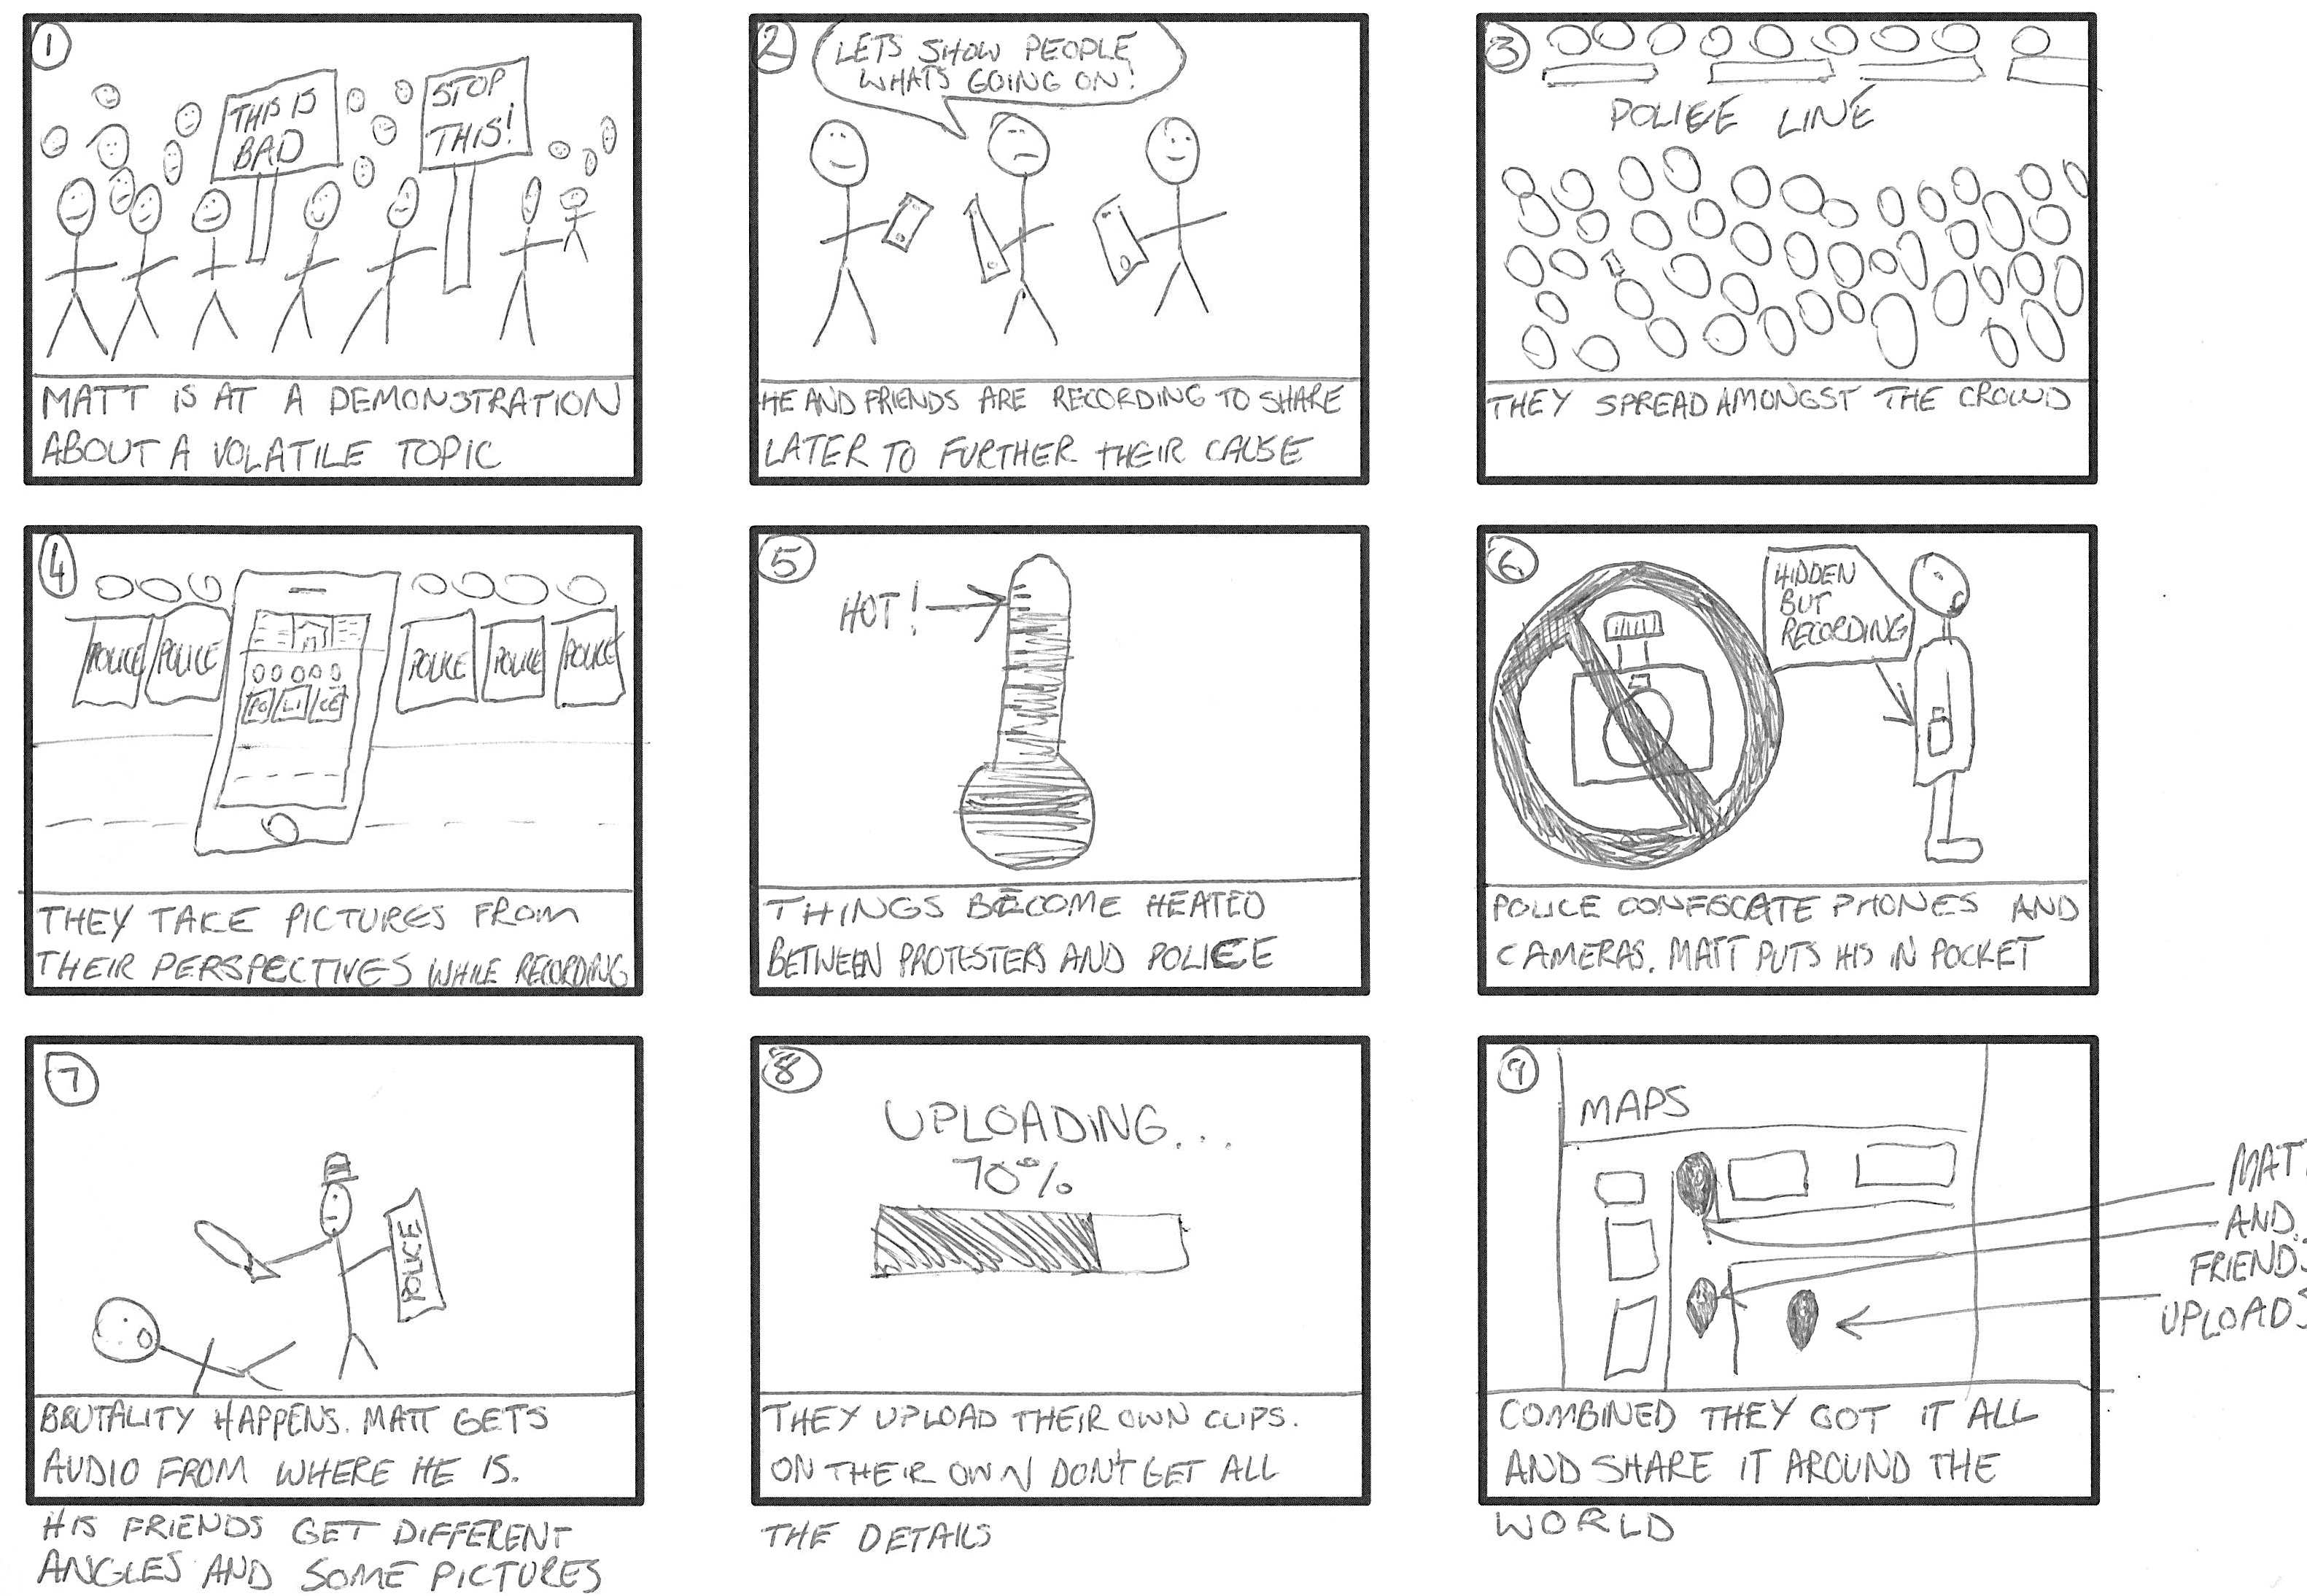
\includegraphics[width=0.75\textwidth]{images/ally-storyboard.jpg}
\caption{An initial storyboard for MDRS.}
\end{figure}

The project's use in public safety was of particular interest to the team. MDRS could serve as a non-invasive and non-threatening way for police officers to monitor an area. It could also hold those officers and those they interact with accountable in a alternative way to current methods such as mounted video cameras.

Include another storyboard here {\bf bold}

From our storyboards we realised that MDRS should be more than an audio recorder with location tracking. By allowing the user to capture images, we could combine these three information sources into a virtual environment that others could explore.

\section{User Interface} The realisation that the project would be spread across
both mobile and static devices raised the need for two interaction models for
MDRS. For capturing the various forms of data a mobile implementation was key. The choice of Android was advantageous in the design stage as it has a flexible framework within which to design an application's interface compared to iOS which is much more restrictive in what is possible. A web counterpart served excellently as the best platform to portray any data collected. Visualising our complex data on a small device's screen would have been limiting. A web gave the team flexibility to take risks and innovate in how we communicated our ideas.

\subsection{Web Application}

%I put this in the wrong section, it really belongs here, I'm an idiot and probably wasted time on this but we might be able to shoe horn it in for extra content

%At the outset of the project the team had planned to build two independent platforms, one back-end server used to process audio and a separate client application to view and amend data. However the team took time to discuss the positives and negatives of this approach; the result of which was decided this was not the most sensible solution.
%The team supervisor suggested we look into Django as a all in one solution, as it provided many of the features this project includes and the team would also benefit from using a simple and also familiar language like Python.
%To be more specific, Django provided the team with built in user authentication, a reliable and easy to use model view controller structure, full database support and integration with the application and the simple fact Django is a web application framework allows the application to be used across almost any device without much regard of portability.

%With this decision made a GitHub repository was made and a skeleton Django project was set up. No-one on the team had used Django before however all members were experienced in Python. A little research was done and a series of tutorials entitled “Tango With Django” was discovered.
%Upon seeing the clarity and level of detail of this document, it was decided to use this as a reference with which to build the web application.
%Team members were given chapter numbers to reach by deadlines; however these were not always met by all team members. The team made progress in learning and understanding how to construct a Django application correctly.
%Once everyone was familiar with the process and details of the Django framework tasks were dealt out and members of the team were expected to achieve certain levels of work each week. However it became quickly obvious that many parts of the application relied on others, meaning one member's work would be held back while another finished theirs. This held back productivity in certain areas of the application, certainly when involving the database and the models associated with it.

%Progress with the web application was steady, the back-end was actually a fairly simple affair in comparison to the front-end which was heavy with scripting.
%Back-end scripting mostly involved getting the models to suit what was needed correctly, it took several trial and error attempts however once the team managed to work out the correct collection of models it was mostly left alone. The only real issue the team ran into was some of the audio formats in the later stages of the project. At the outset OGG was decided as the format to use as it had a great compression to quality ratio; however it was discovered that Android could not, in fact, encode audio to OGG directly. Since a majority of the web code had already been written a decision was made to simply take a format Android could encode in and then convert it to OGG upon upload to the server.

Given the nature of MDRS, the team looked to the Distributed Information Management course taught in second semester as a source of possible tools. The course is structured around the use of Django, a Python based web framework which we considered  would offer us the flexibility to create a rich, dynamic application easily deployable to possible users. Widely used, Django had a wide range of support materials available including Tango with Django written by Leif Azzopardi and Glasgow University postgraduate student David Maxwell. This resource and knowing we would have to learn it later through coursework made the framework choice an easy one. It helped to solidify in the design stage how the team could retrieve the data to then present.

\begin{figure}[ht!]
\centering
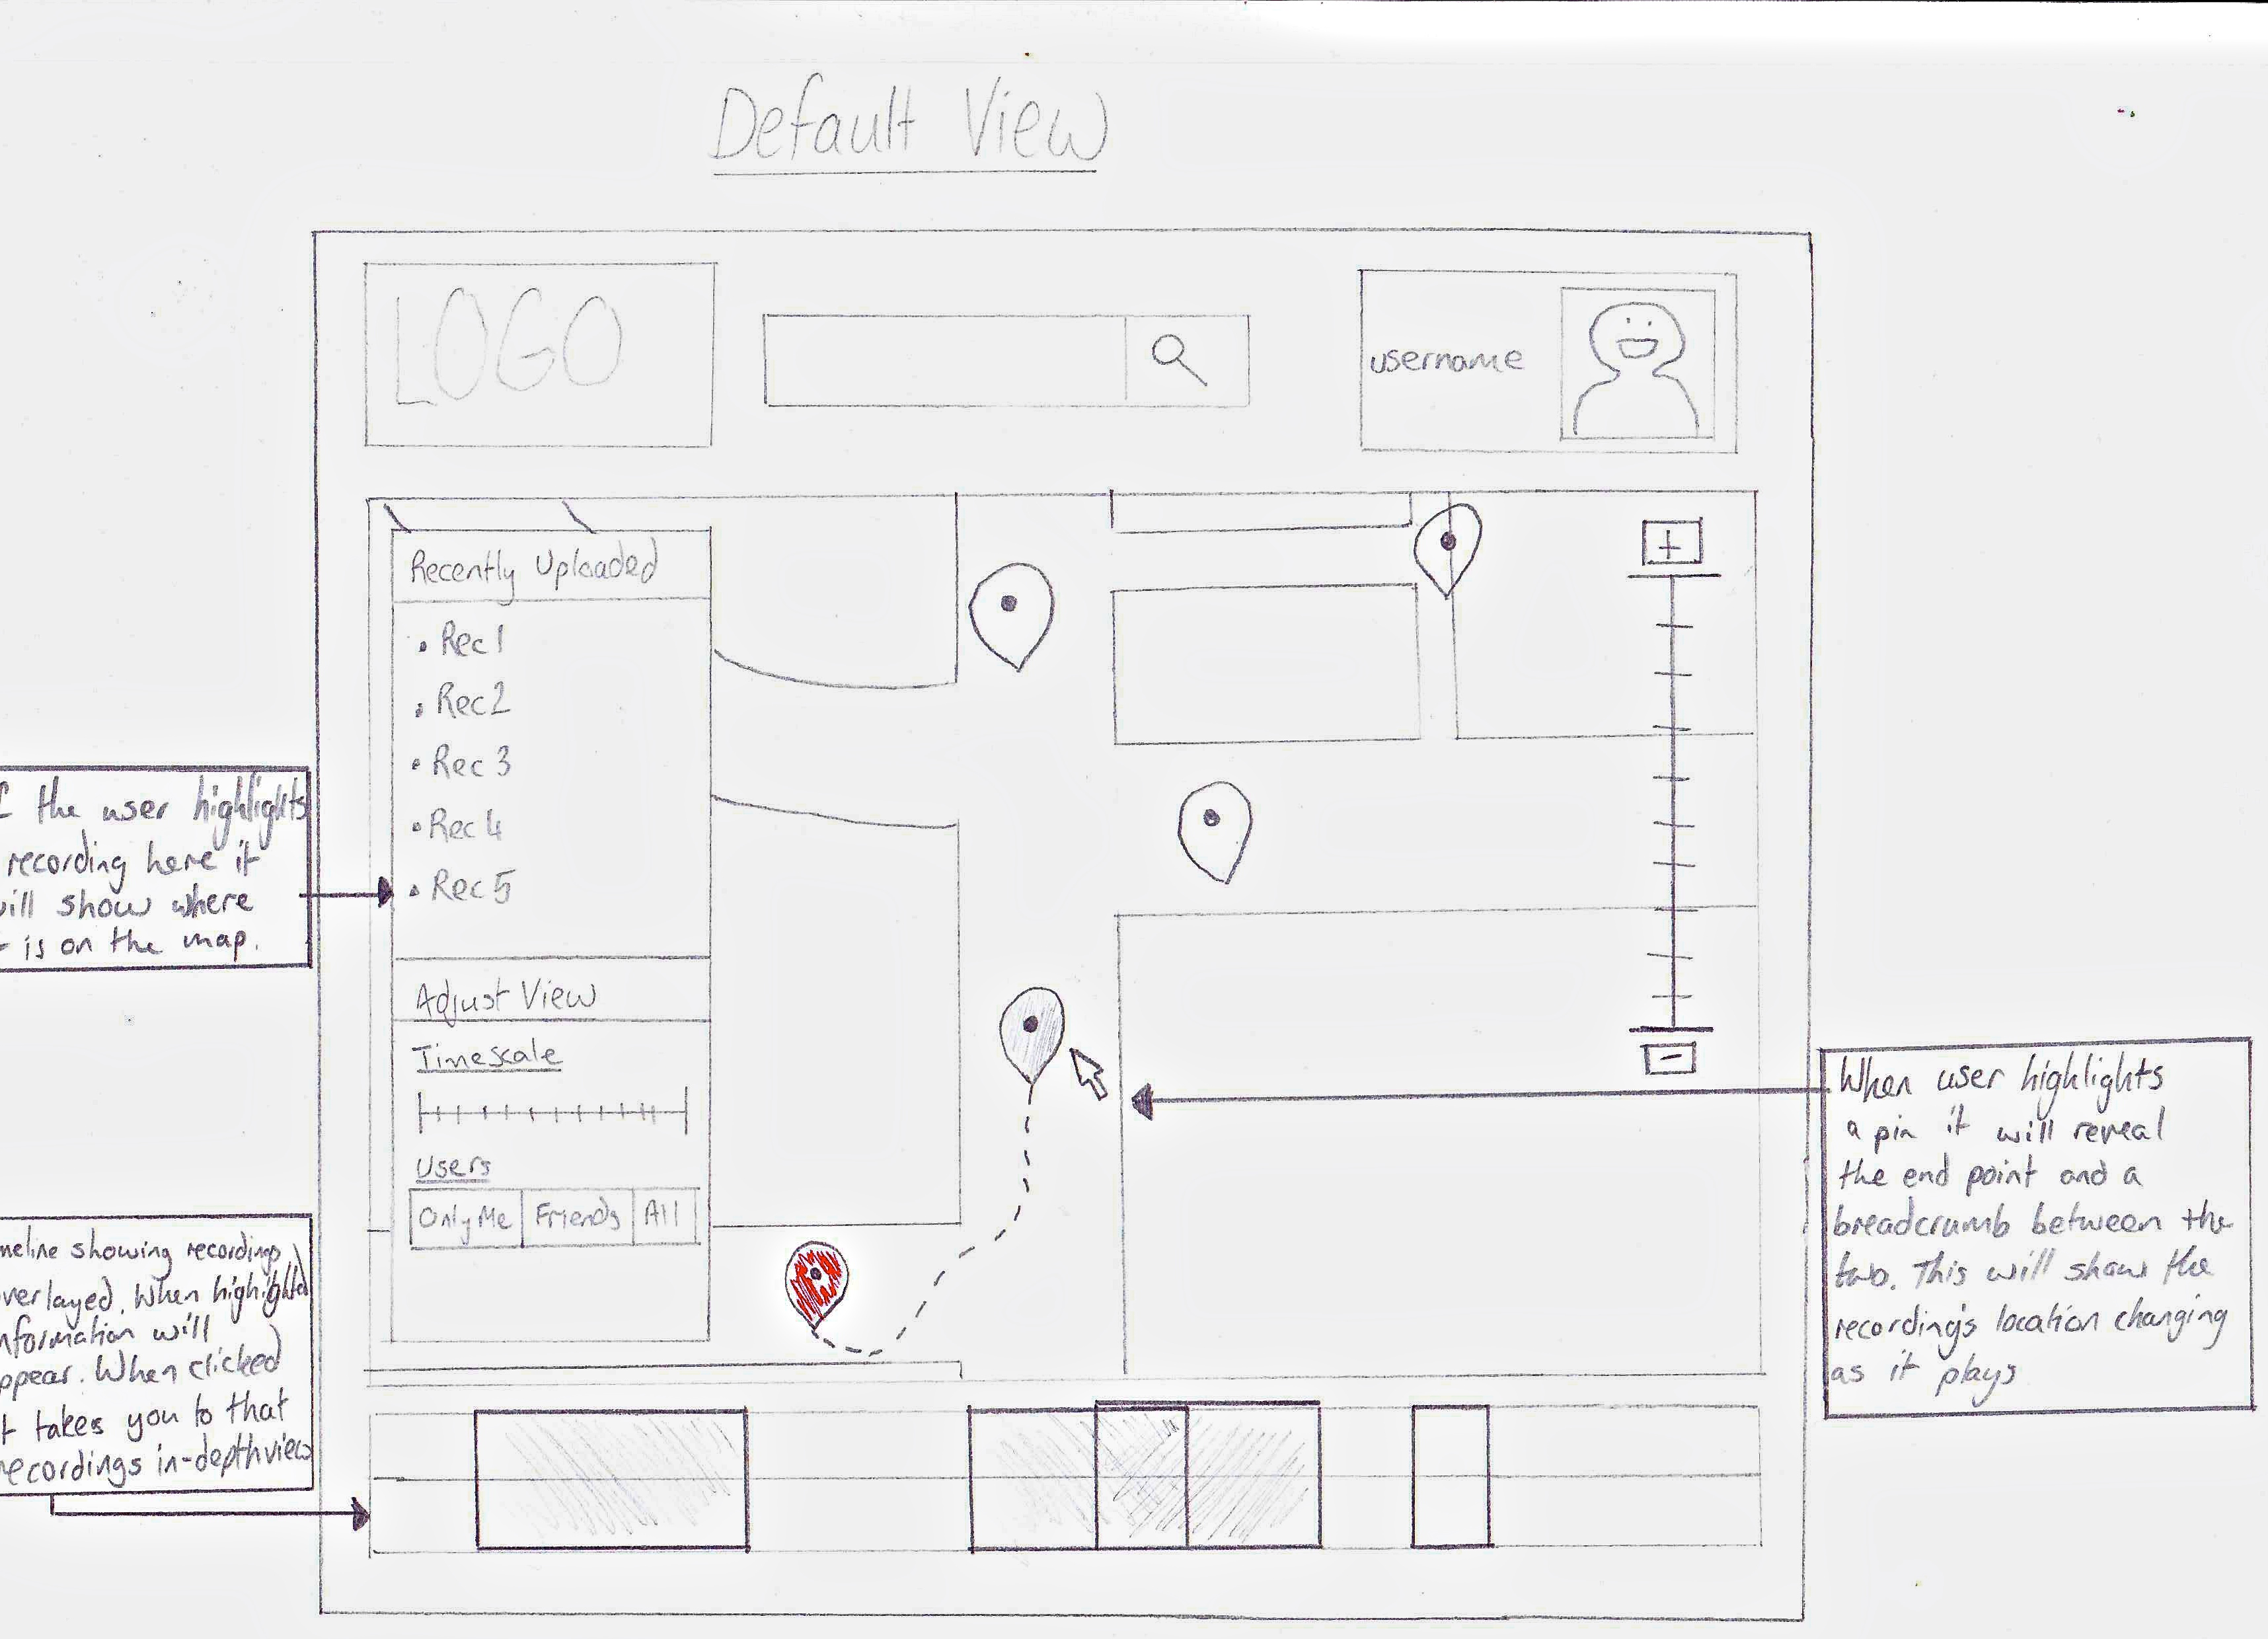
\includegraphics[width=0.75\textwidth]{images/web-map-view.jpg}
\caption{Prototype of map view.}
\end{figure}

The key interaction between the user and MDRS is location therefore it made sense to make a map the central interface. The user would be able to explore the map and click on pins representing recordings. This would then project the path of the recording , 'lighting the way', indicating where images were captured along the way. Users could then play it back individually or select multiple recordings for synchronous playback. With such an important role, the importance of which mapping API to implement was extensive during prototyping.

Our choice of Google Maps was immediately found to be the correct one while prototyping our interface. The simple API made it easy to test out different styles of visualising recordings. To get these prototypes off the ground all the team needed to do was  reference the Javascript library in the HTML file. After multiple tests it was decided that a custom marker would mark the beginning of each recording. Once clicked on, this would trace the route of the recording, showing its terminus. While earlier approaches showed the paths all the time, this cluttered the interface. Another test tried having the map blank to begin with and only populate as the user chose their recordings from a list. This was found unengaging and the team felt users would lose interest without visual stimulation as soon as the page loaded.

Alongside our relatively simple use of maps, we prototyped a version which would incorporate Google's Street View. This would allow the user to follow a recording's location trail even more closely. By harvesting the orientation of the recording device we could show where they were looking, showing the Street View at that angle, and overlay any of the user's own images they captured on top of this. While this immersed the user even deeper into the recording, it was unfortunately not taken beyond this prototype stage due to the complexity of implementation required.

\begin{figure}[ht!]
\centering
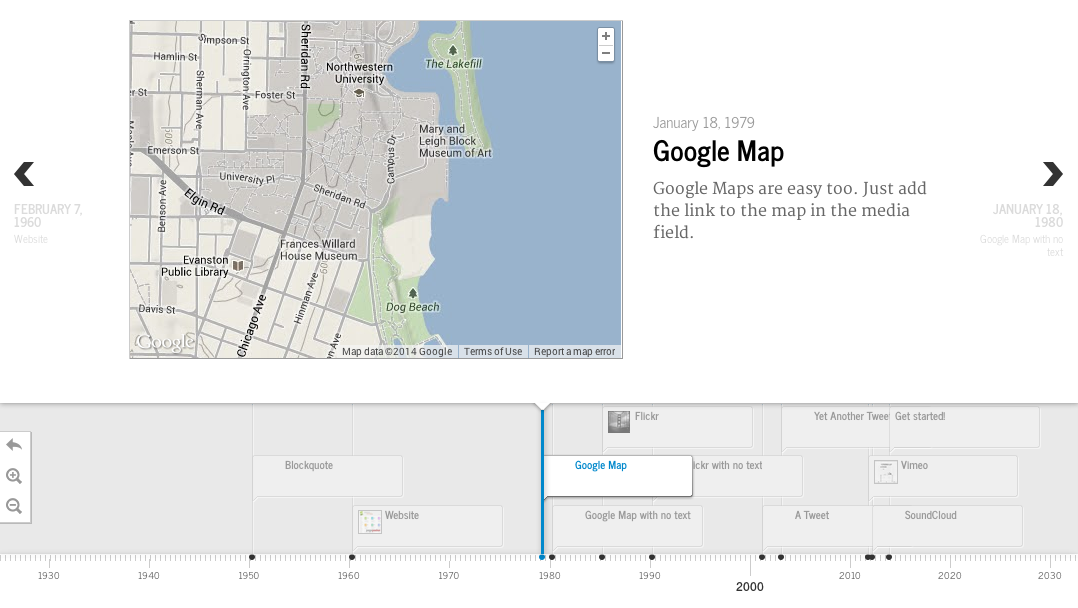
\includegraphics[width=0.5\textwidth]{images/timeline-example.png}
\caption{An example of TimelineJS by KnightLab.}
\end{figure}

A second key component to this interface is the interactive timeline. This was hoped to show the length of each recording and where they overlapped. Upon clicking on a recording, a dialog would show its metadata such as name, description, the user who captured it and any accompanying images. In earlier prototypes the ability to scrub along the timeline was included. This was removed as no Timeline researched offered the functionality.

Early web interface designs featured a prominent header bar and a floating menu panel which moved over the map. From early prototypes and wireframes this was realised to waste a lot of screen real estate, detracting from the reason the user was on the website. The header bar in particular became wasteful as the ability to search all recordings was downgraded in importance within the application. Through discussion in the team it was decided that users would more likely be interested in audio based on location (the key paradigm of MDRS) rather than searching through keyword. It gave us a stretch goal to aim for if development moved along smoothly. PureCSS' simplicity favoured our team's limited prior experience with web design. The elements included in the toolkit all look great and gave a lot of direction in how to integrate navigational controls.

\begin{figure}[ht!]
\centering
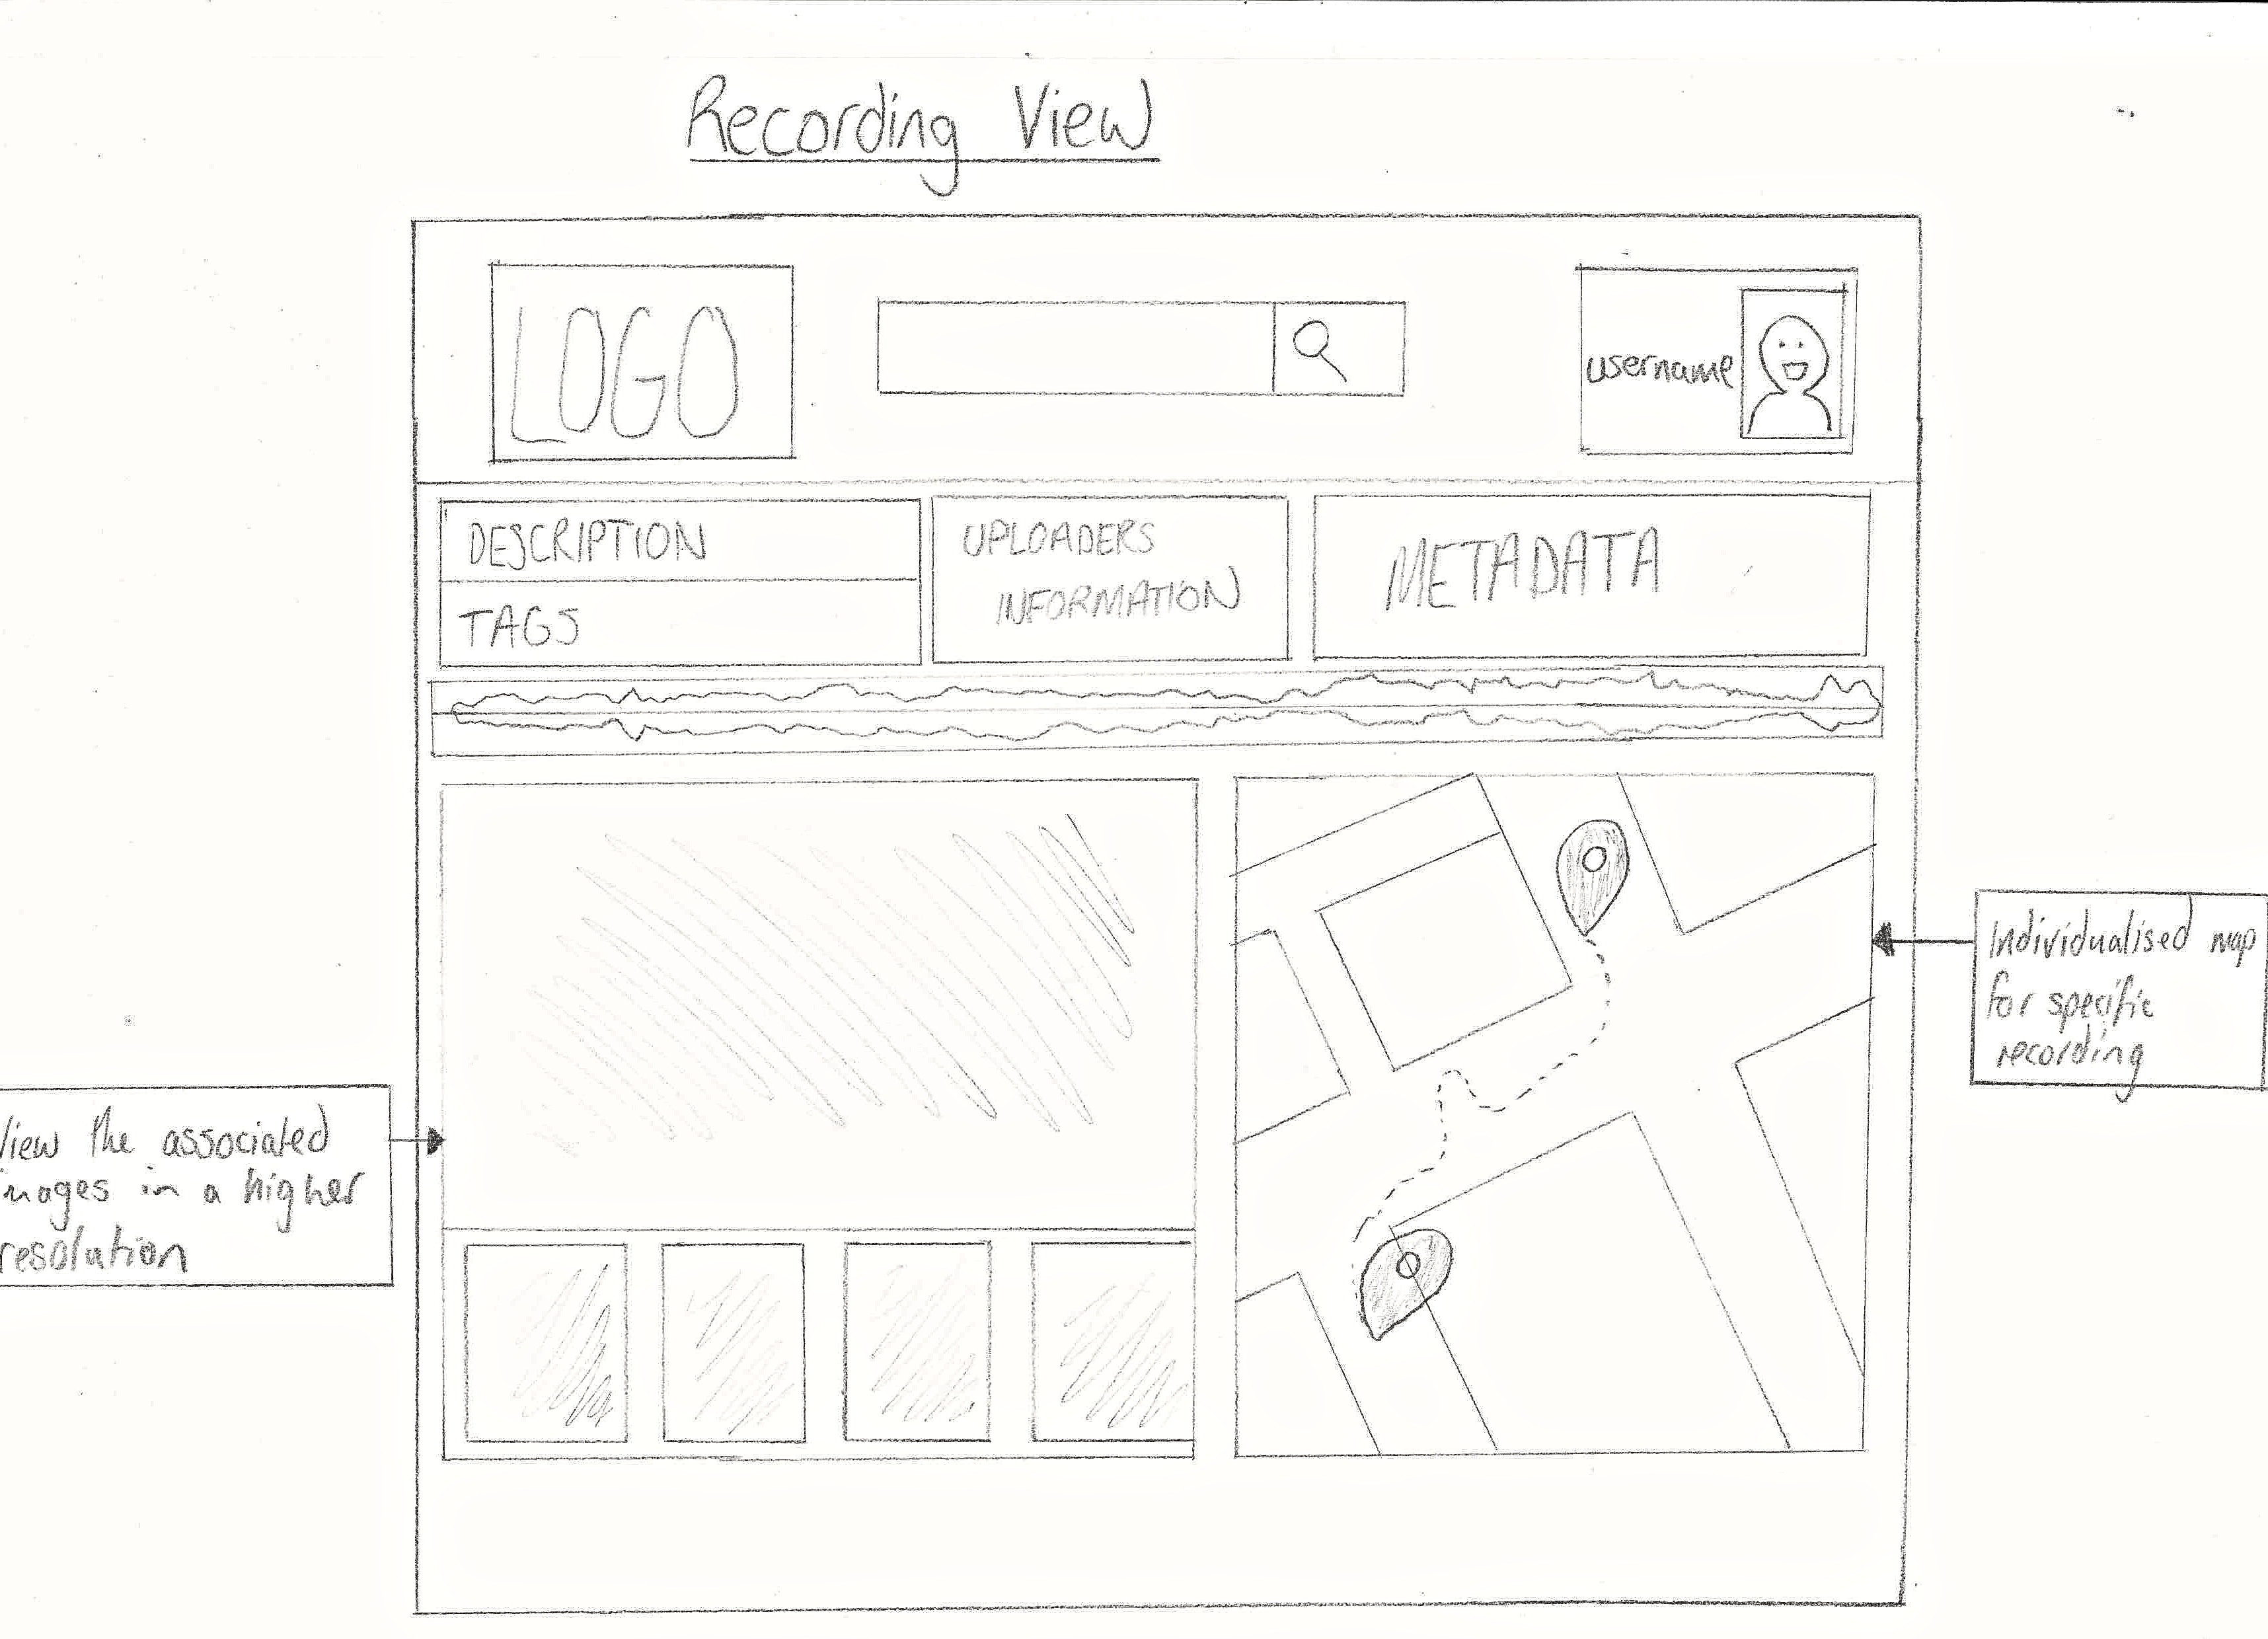
\includegraphics[width=0.5\textwidth]{images/web-recording-view.jpg}
\caption{Recording specific prototype for web application.}
\end{figure}

To accompany this main map view of MDRS was a user page which offered a
personalised insight into a user's recordings and activity with the application.
It included a personalised timeline and map showing their personal contributions
to the map from which they could play, edit details or delete them from the
service. Along with all the other tools mentioned, the foundations of our
web application's design were laid.

\subsection{Android Application} It was decided early on to approach this
element of the project realistically and working from a simple set of requirements to
make the application easier to implement. This would allow us to make the user experience focused on the core of MDRS, capturing information from the world around us. This meant it was purely a capture and upload system and it wouldn't be an alternative to the desktop viewing interface for interaction with other user's recordings. Our focus made the application more achievable while leaving scope for extension in future development for these playback features.

To develop an engaging user interface on Android, the team looked for a scalable and intuitive design, drawing influence from a wide range of applications such as Foursquare, Snapchat and Google Play’s suite of applications. Google's Android Design Guidelines were consistently referred to throughout this process for inspiration.  Foursquare's integration of a map into a larger whole was seen as an excellent touchstone while Snapchat's unconventional, yet intuitive navigation model was seen as a strength of the application the team could borrow from. Google's applications portrayed the strength and beauty of clear typography and the undeniable rule of mobile design where less is more. Sources such as Android Niceties were also used to find innovative design that could help with MDRS. A utilitarian minimalism through design was the team's goal. The core functionality of the application was single use and the flow through it was clear, allowing for a relatively simple approach to be taken, finding a place for flair within the constructs the team placed on themselves.

\begin{figure}[ht!]
\centering
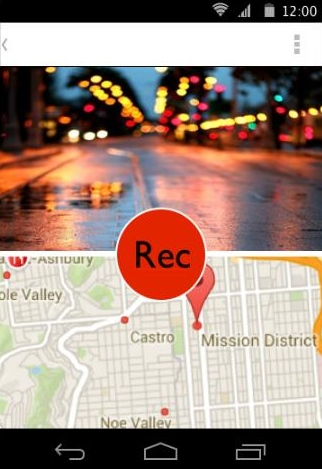
\includegraphics[width=0.34\textwidth]{images/android-digital-prototype-1.jpg}
\caption{Intial Android interface design.}
\end{figure}

This first UI design offers a split with both a map and view through the camera
lens. The influence for the central record button came from Foursquare’s
prominent placement of their check-in button, placing the key functionality
centrally to draw attention. The downsides to this were its limitations across
smaller screens and a confusing interaction model. Could a user interact and
capture an image before hitting record? This lack of clarity lead to a
revisionary second prototype.

\begin{figure}[ht!]
\centering
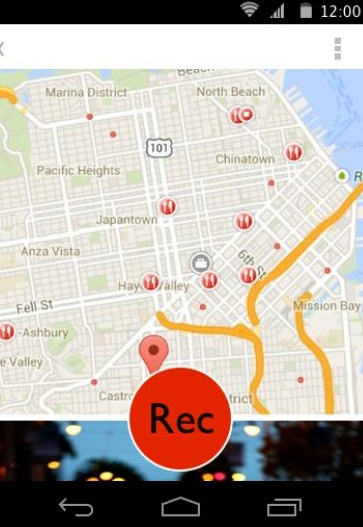
\includegraphics[width=0.34\textwidth]{images/android-digital-prototype-2.jpg}
\caption{Second Android interface design iteration.}
\end{figure}

This prototype drew more influence from Snapchat’s sliding interface, replacing
its horizontal movement with a vertical one. Again showing the record button on
the divide between a map and camera view, once the record was initiated the map
would slide up bringing up the camera view which would reveal from behind a
frosted glass effect the user's view into the world they were recording,
prompting them to capture images.

While these both informed the team in the direction of the application's design some aspects such as the sliding divide between map and camera were removed to accomodate a clearer path the user could follow through the application while simplifying the implementation required.

\begin{figure}[ht!]
\centering
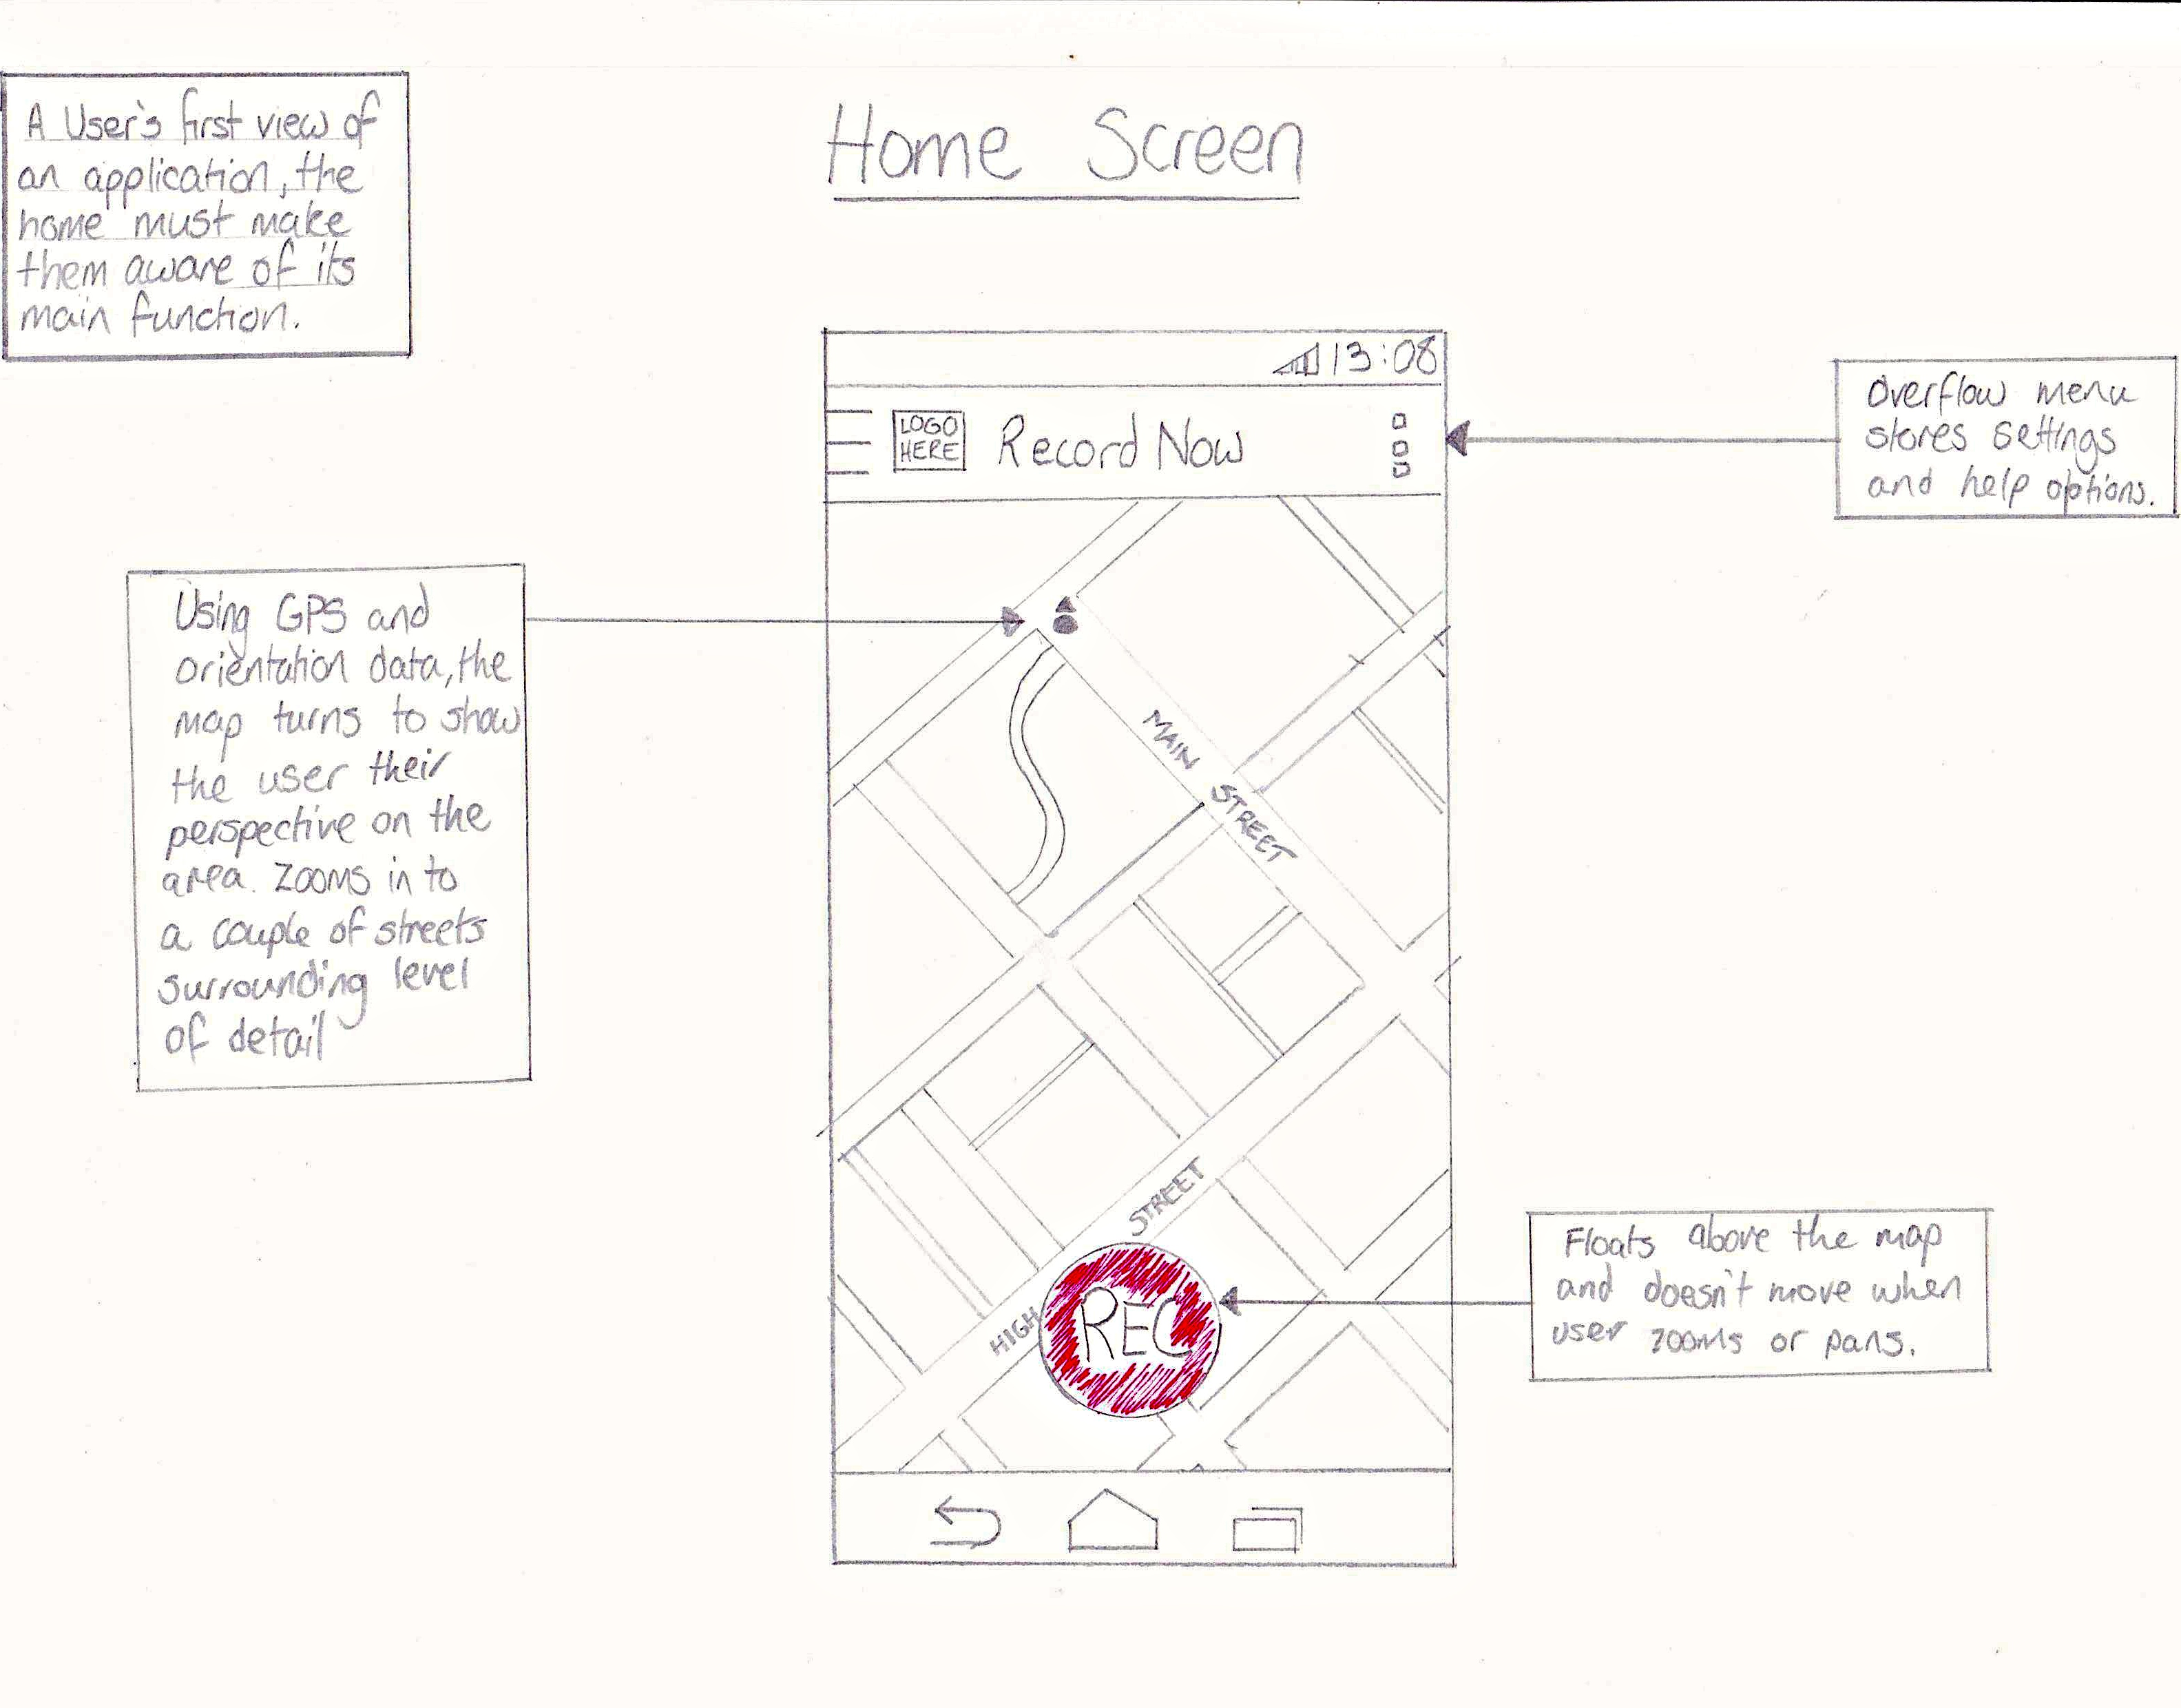
\includegraphics[width=90mm]{images/android-home-view.jpg}
\caption{Final design prototype}
\label{overflow}
\end{figure}

This final design exudes simplicity with a single actionable button on the main view. This was to allow MDRS to blend even more into the background. The application's aim was to capture its surroundings while reducing the user's interaction with their device to a minimum. The map would automatically centre on the current location and indicate the user's orientation. Briefly the team considered if the map would rotate to match the orientation but it was felt an unfamiliar perspective on a map traditionally viewed oriented north could confuse. It was decided the marker's directionality would be enough of a suggestion.

\begin{figure}[ht!]
\centering
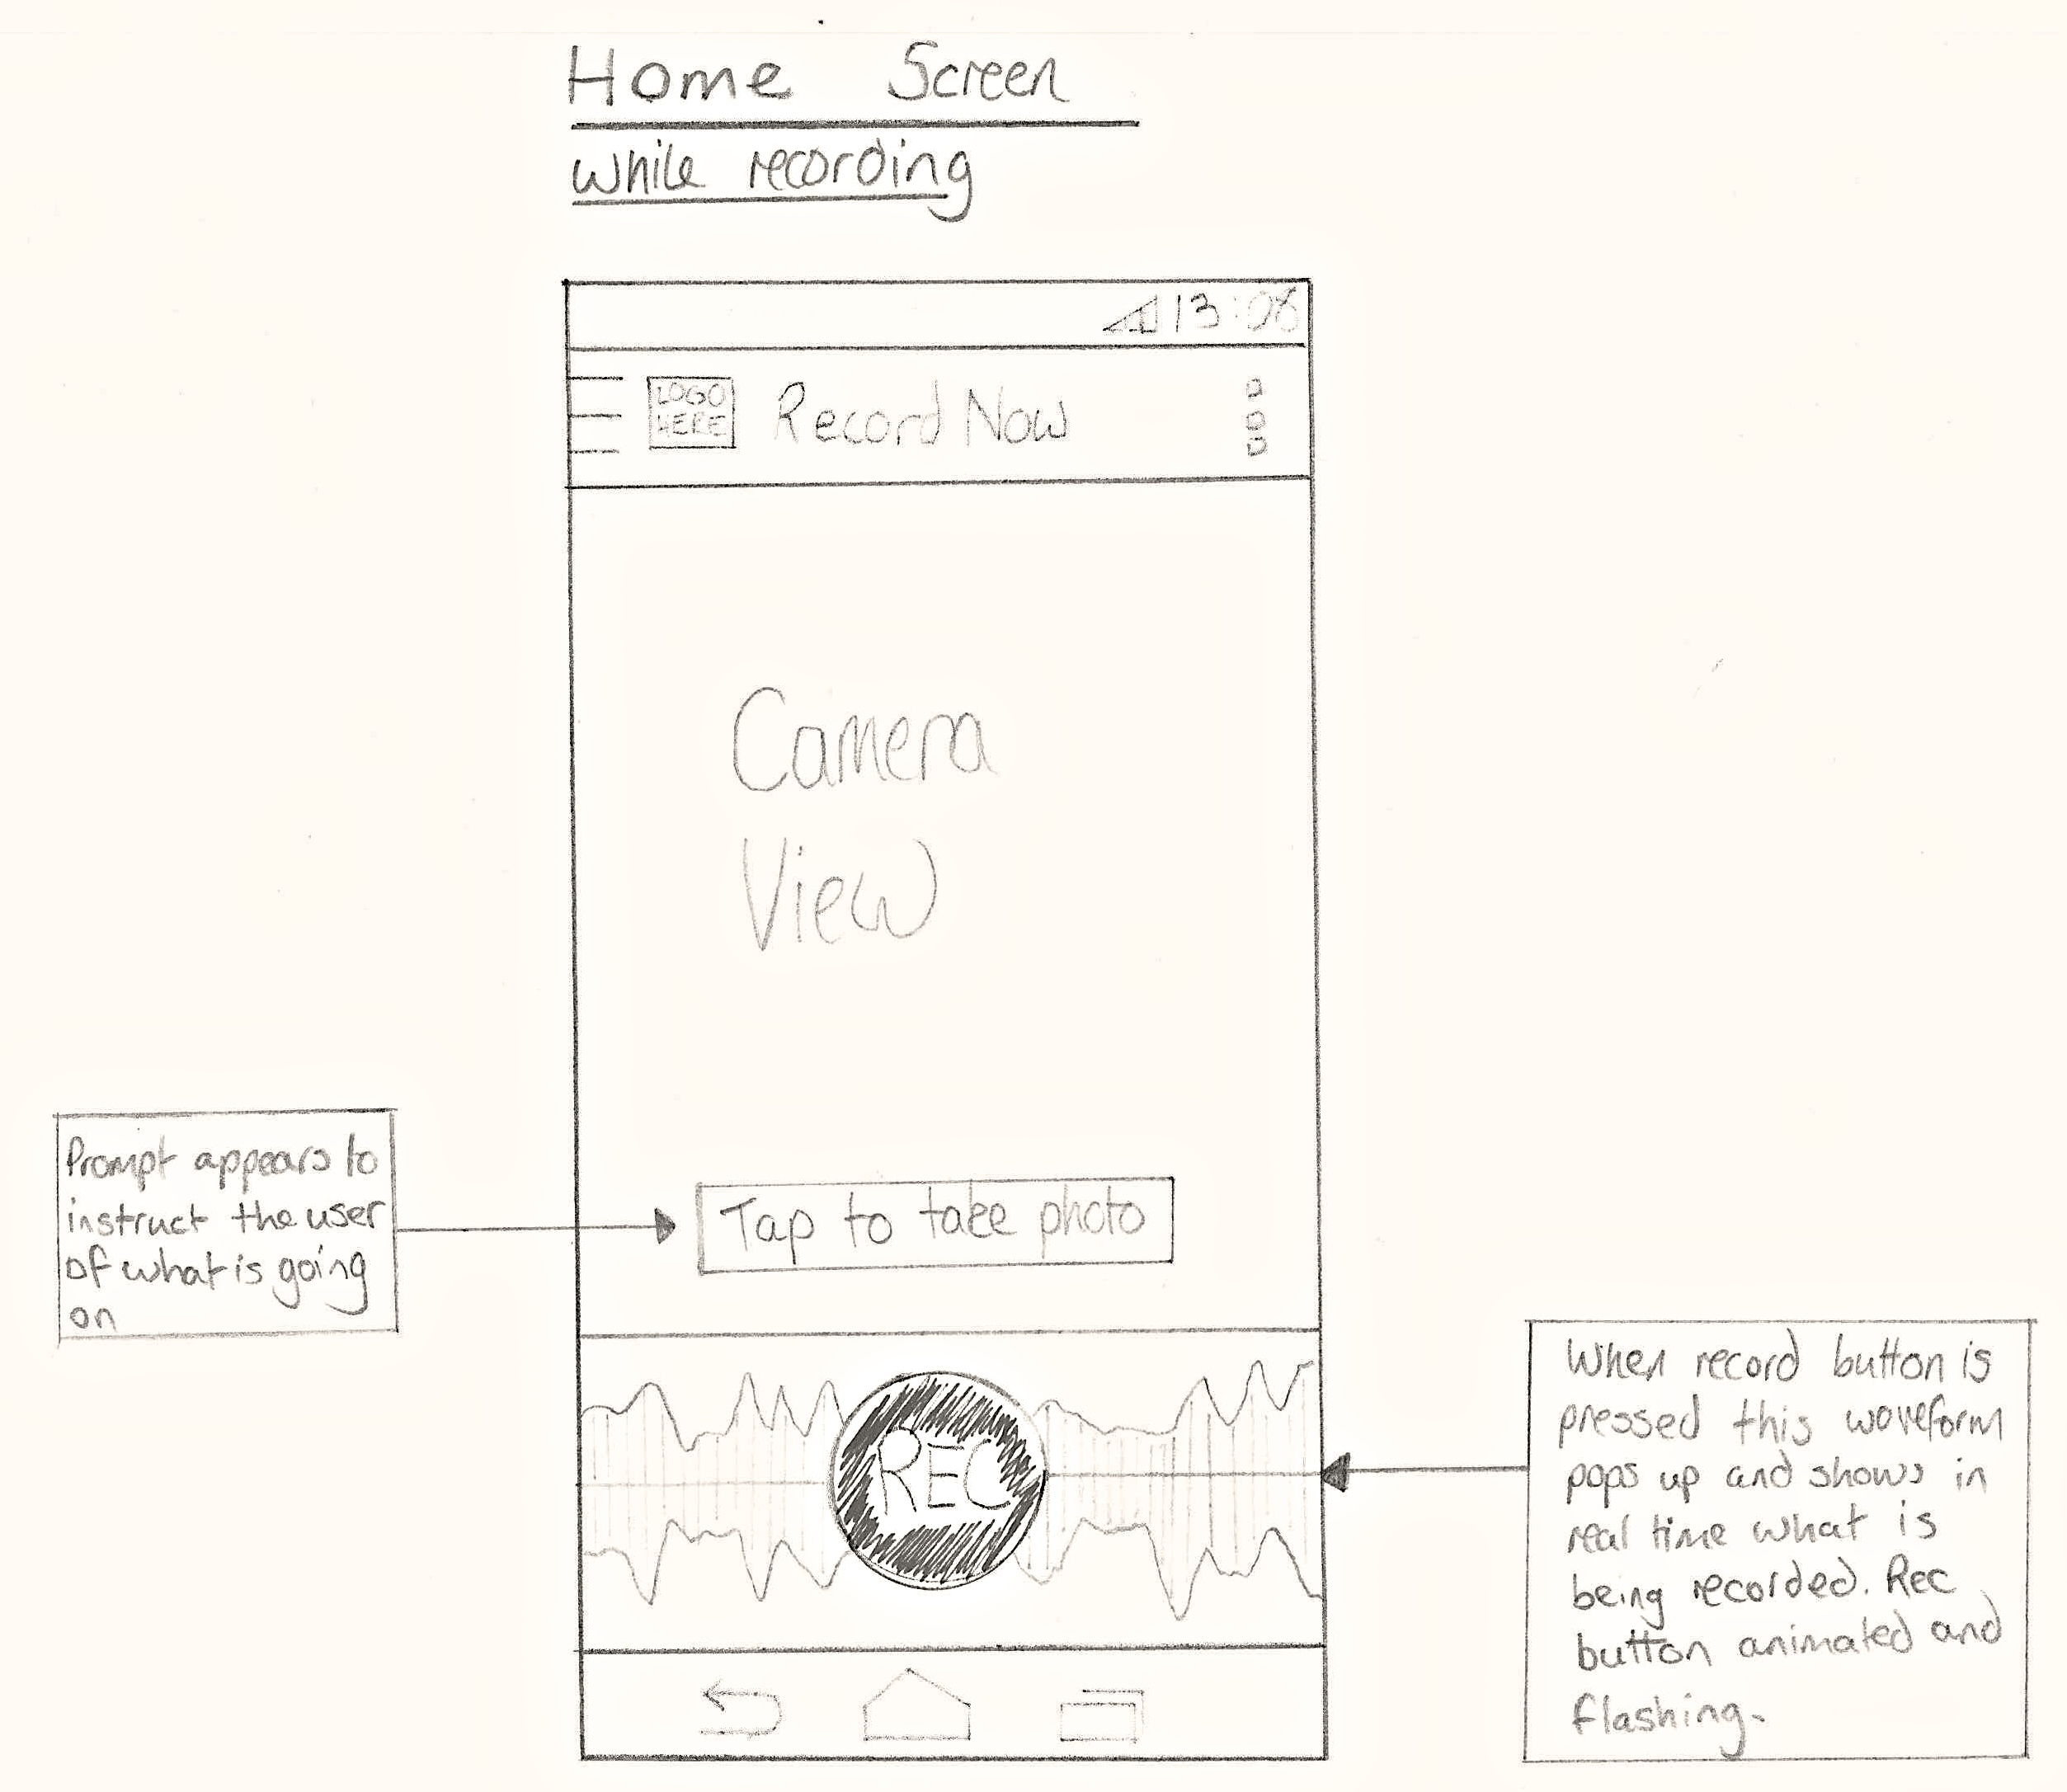
\includegraphics[width=90mm]{images/android-recording-view.jpg}
\caption{Recording view of final prototype}
\label{overflow}
\end{figure}

When the record button was pressed the entire screen would transistion to this view. Every detail was included to inform the user of the application's intent and current state. A brief notification would alert the user that they could capture images by clicking on the viewfinder. A soundwave visualisation demonstrated that audio was being captured and the map on the previous screen was intended to make the user aware that they position was being followed.

\begin{figure}[ht!]
\centering
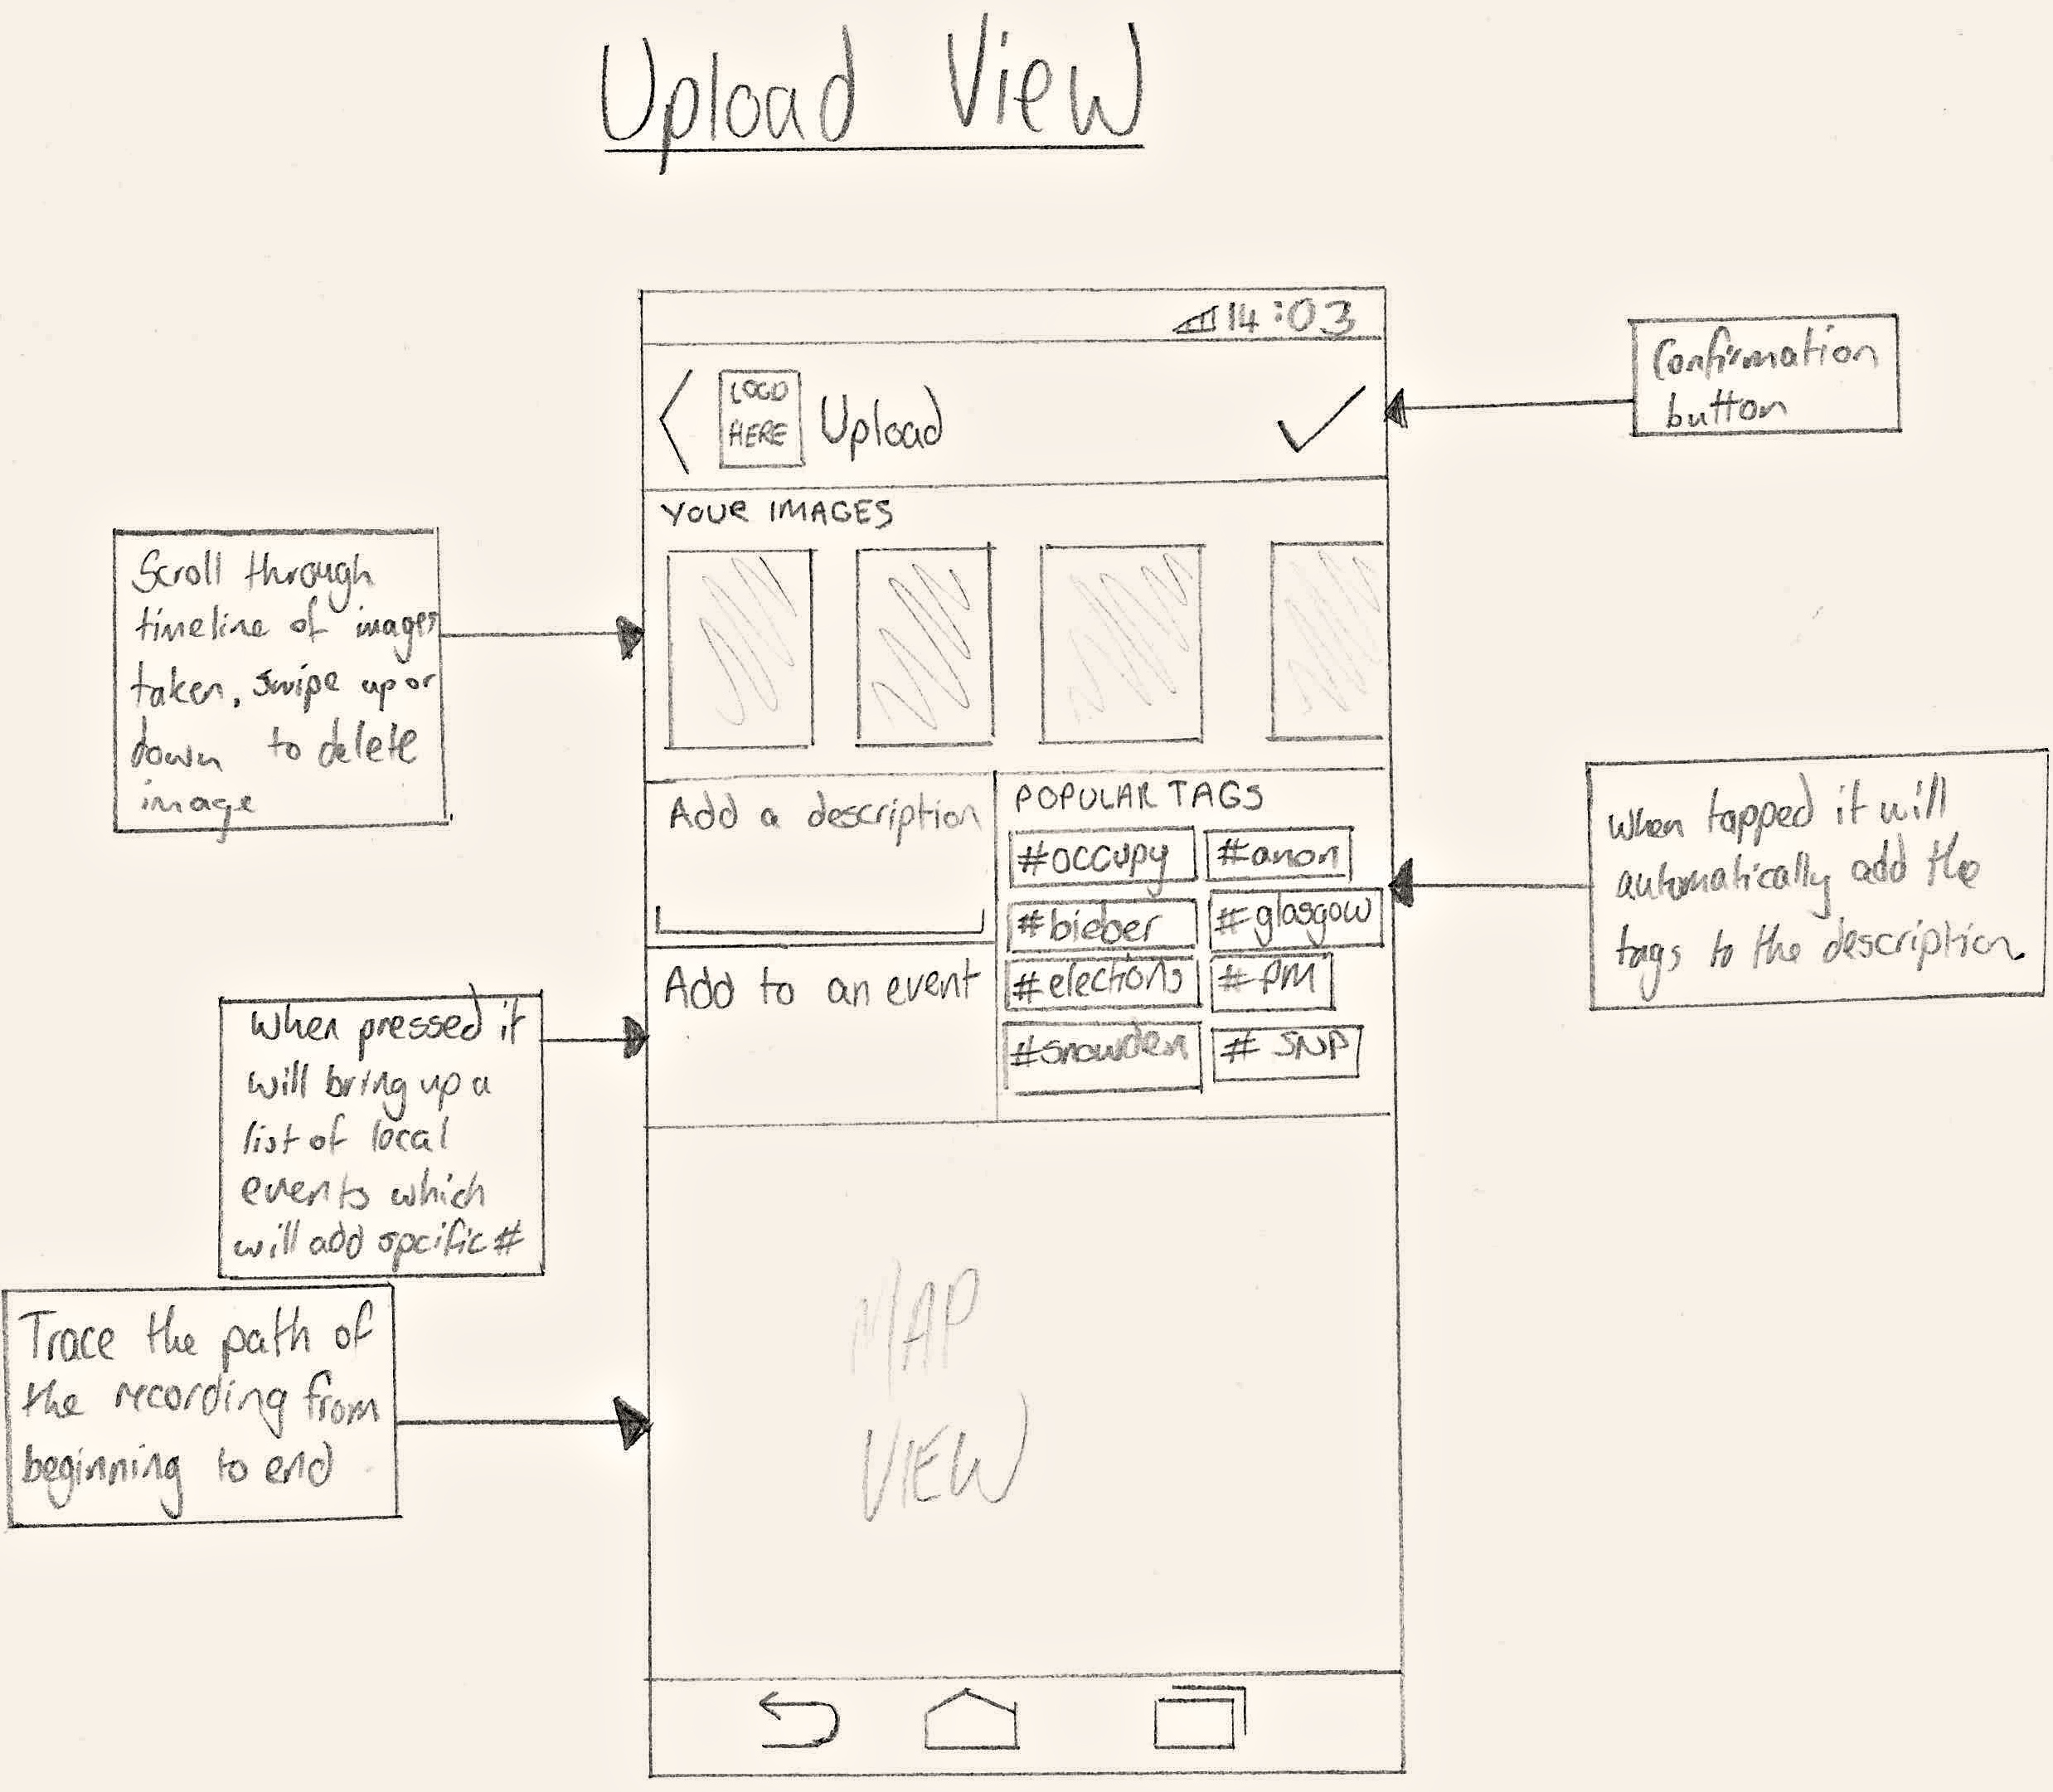
\includegraphics[width=90mm]{images/android-upload-view.jpg}
\caption{Final upload view prototype}
\label{overflow}
\end{figure}

Finally the upload screen informed them of their path through the map view. The option was then given to define their recording with metadata such as a title, description and tags. These three separate views informed the final implementation extensively and aimed to create an intuitive experience for the user.
%==============================================================================
\chapter{Implementation}
\label{impl}

\subsection{Server and Django configuration}
Being granted use of a university server, the team had a server to base all of their work off of. One team member was given the task to set-up and maintain the server.
Set-up was a simple case of installing the necessary packages from the \gls{Ubuntu} repositories such as Git, Python, Django, \gls{PIP} and \gls{MySQL}. After downloading and installing packages some configuration had to be completed. This mostly involved setting up user accounts for each team member, a shared workspace for everyone to work in, set up permissions and make sure every member had sufficient access to all the needed tools.

This, having been completed, lead to cloning the team Git repository to the server. Some permissions teething problems were immediately encountered as some members could not edit files. However these were minor issues dealt with some basic configurations.
Having the file set now on the server it was a simple case to initialise a database for the project and get it to a working state. However there was immediately an issue in that regular users could not host the server on port 80 (the standard port for HTTP requests and the server's only open port) without administrator privileges. This meant that each team member would need to login as our shared super user account to simply run the server; this slowed workflow and so a solution was devised. By manipulating the IP tables on the server, the team successfully managed to route port 8080 internally to port 80. Simply put this meant the team was fooling the server into thinking it was hosting harmlessly on port 8080 whereas it was getting rerouted, after the user invoked the command, to port 80. Exactly where the team needed the socket bound to.

Later issues appeared as development continued, many of them minor issues such as the database needing reinitialised or the server rebooted and the IP tabled reconfigured. All issues were dealt with swiftly and with little to no impact to the development of the project.

\subsubsection{Django Configuration}		Having no experience with Django before this project, the team had to rely heavily on the 'Tango with Django' book to understand and continue with development. When it came around to configuring the server there was little to no resistance however. A lot of the Django settings and configuration is boilerplate.\footnote{These parts are uniform across many applications with few custom settings required for MDRS.}

The team made the initial decision to split the application into two sections. The main section, simply titled after the project MDRS, contained the settings and main routing Python files. The second section, entitled web app, dealt with all functionality of the application. Web app contained scripts for routing requests, parsing them, passing back templates; also dealing with all POST requests and file handling.

The configuration involved in this was minimal, simply using the manage script the team created the web app partition and began work straight away. As development continued only minor edits had to be made to the settings of the project. One key edit made was to include the session cookie plugin to allow users to log in and maintain their sessions correctly.

\section{Web Application}		During development worked required for the web application was separated into discrete parts. With team members working across these parts spread the work effectively. When extra help was required, another team member would assist the current 'specialist' of a feature. This for the most part didn't cause any issues due to effective communication between the two developers. This was usually done using GitHub Issues or more informally through Facebook chat or 'face-to-face' communication.

\subsection{User Interface}		The UI went through a number of iterations during the the development cycle. The early interface was built from the ground up causing innumerable problems, this was down to a lack of experience in web design by the team members. Once a PureCSS alternative was put in place, the development's pace recouperated and continued.

It was the aim when approaching the UI to achieve a consistency in the colour scheme and layout throughout the application to promote ease of use. Buttons and options were kept to a minimum and functionality was designed to be as clear and intuitive as possible.

\begin{figure}[ht!]
\centering
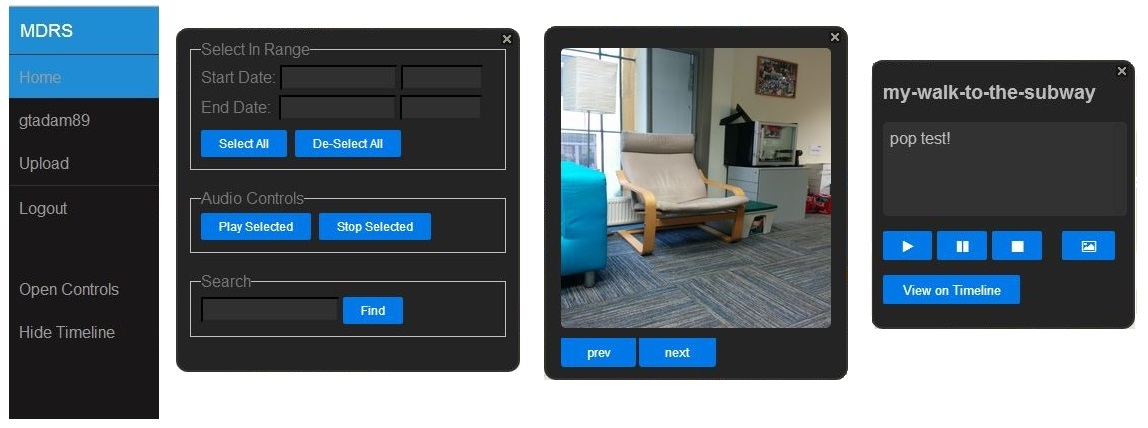
\includegraphics[width=0.95\textwidth]{images/ui-elements.jpg}
\caption{Navigation Menu, Control Box, Picture Box and Recording Box}
\end{figure}

\subsubsection{Navigation Menu}		PureCSS was leveraged for the navigation of the web application. By using the framework we saved a lot of development time to focus on other areas. Earlier on in the development all the UI controls were located within the navigation menu, however it became quickly apparent that this would create an overly cluttered and unprofessional appearance. So the controls for the map were relocated to a separate box, and a button opening the box was located within the navigation menu. This button also changes it's text dynamically relative to whether the box is open or closed.

This menu also utilizes Django's object relational mapping (ORM), so that if a user is logged in, their username would be displayed on the menu as a link to their profile. This personalisation was hoped to make the website easier to navigate, clarifying that link's function. The current page is also highlighted in the navigation menu, to improve their navigation around the application. A button in the menu allows the timeline to be hidden in case the user wants to completely focus on the map.

\subsubsection{Control Box}		Another feature created to keep the interface simplified was the control box. This dialog holds a number of controls over the application as a whole. The control box is separated into three logical sections; 'Select in Range', 'Audio Controls' and 'Search'. Only including options that were useful and could meaningfully modify the data was key in the construction of this dialog. For example in the 'Select Range' section if the start date is left blank it is assumed that all dates prior to the end date are desired. The opposite is true for end date, however if both dates are left blank all are selected. To create options for this in the box could lead to a more complicated UI though it proved unnecessary to do this as these features were intuited by most people during testing.

\gls{JQuery} Datepicker was used as the user interface for selecting a date with great success, the colours were edited to give a more consistent appearance and integrated feel. Originally when a date was selected it came up in the American format, though this was easily changed by using the documentation provided with the JavaScript library on GitHub.

During internal testing, the team realised filtering by date alone was not enough as the scope of recordings narrowed down to could still be huge. It was decided to use JQuery Timepicker for selecting a time. This timepicker has a similar appearance to that of the timepicker on Google calendar.

The second section in the control box 'Audio Controls' offers the ability to play multiple recordings all at once, this feature utilises 'Buzz!' and its support for grouping multiple audio files together. This feature works by using the earliest recording in the group of selected recordings as it's datum, from there all other recordings are synchronised. This approach has it's drawbacks, though a more intuitive system was not an option due to the limited timescale imposed on the group.

Finally the third section is 'Search' this allows the user to search for a recording using the name of that recording. This functionality unfortunately was found, during testing, to not scale as well as we might have hoped. This was down to the fact that if you did not know the name of a recording there was no other option offered to find it. Options that could have been included may have been such things as tags or by user. There was also performance issues, as it took all the recordings from the database for the autocomplete no matter what was entered into the search bar.

\subsubsection{Recording Box}

This box displays the metadata associated with the recording that has been clicked. The colours chosen were picked to fit as closely with the sites theme as much as possible. If the description is too long to fit into to the description box it displays a custom  scroll bar. It should work in most modern browsers though degrades gracefully if it is not supported. There are a number of buttons in this box each with a separate purpose.

The first three buttons are audio controls for 'Play', 'Pause' and 'Stop'; each are represented by the usual symbols. These buttons utilize 'Buzz!' for playing the recording associated with the record currently loaded in the box. The next button in the box is one that allows you to load the Picture Box, this is represented by an image icon on the user interface.

Finally there is a button for viewing the position of a recording on the timeline, as there can be any number of recordings on the timeline all at once, to do this manually would be infeasible. So when the button is pressed, the timeline will scroll to the recording loaded in this box and will be selected on the timeline.

\subsubsection{Image Viewer}		The image viewer was kept simple with next and previous buttons the same as the rest of the buttons in the user interface, this box displays all the images associated with a recording. It uses SlidesJS \footnote{SlidesJS is a plug-in for JQuery} which  allows you to view images in a slideshow format.

There was a number of issues during development of this feature as dynamically changing the images in the slideshow was not something supported by this plugin. However this was neccessary in order to change the images when a different recording was selected. Workarounds were unfortunately put in place to get this feature working, however inelegantly on the backend, due to the limited timescale.

\subsection{Map}		A number of technologies were used when implementing the map and they all had to work in harmony to effectively display to the user the recordings that were stored in the database. The major components were Google Maps, HTML5 Geolocation and JQuery. Combining these allowed the team to create a meaningful visualisation of recordings captured.

\subsubsection{Map API}		The Google Maps API was used extensively throughout the development of the home page with many of the Javascript classes and objects used. On the Google Maps API website there was many examples given showing how these could be used, these resources were invaluable during the development process, especially during the early development process allowing rough prototypes of certain features to be created with very little trouble. The map was initialised using,
\begin{verbatim}
google.maps.Map
\end{verbatim}
For the appearance of the map a few simple changes were made such as removing certain UI elements that come with the map as a standard. For example it was decided to remove the \textit{Pegman} icon as we would not be incorporating street view into our initial product and the presence of this icon could prove to be an unnecessary distraction. The zoom controls and slider were also removed.

After having created an instance of the map and styling it correctly, we were then able to receive the bounds of the map displayed on the screen, using the method:
\begin{verbatim}
getBounds()
\end{verbatim}
This was important as from this we were then able to query our database using JQuery (this method will be covered in a the JQuery section) and receive from the database only the recordings that would be currently visible on the timeline. For were we not able to receive the bounds of the map and just all the recordings were returned, this would prove a serious problem in scalability.

These recordings were then plotted on the map by creating multiple instances of the marker class for each recording. These markers must be created using the object:
\begin{verbatim}
google.maps.LatLng
\end{verbatim}
In this particular case this object is being used as the latitude and longitude of the marker, which is created using the data that has been returned from the database. The co-ordinates that are used are the start position co-ordinates of the recording. We decided to use a custom icon for the default marker to give a more consistent theme, also in order to differentiate between non-selected and selected markers a separate red version of the marker was used.

The behaviour of the markers had to be defined manually this was done using JavaScript. An example of such behaviour would be if the map was panned and a recording fell outwith the bounds of the current view then this pin would be removed, and then added back in again if it is brought back in to view. It was an initial requirement that support for the "selection" of multiple recordings must be incorporated into the map so that these recordings can then be played back in a synchronised form. What was written allowed a pin to remain selected even if it was not currently in the view of the map. In other words when a pin is selected it would be saved in memory until such time as it was deselected.

Originally the google maps info window was used to display the metadata to the user, however in the late stages of development this approach proved to be inflexible as any minor changes to the appearance or positioning of these info window’s would prove to be overly complicated. In particular through testing it was discovered that it was routinely obscuring the route of the recording, as a group it was decided to place it in the top right hand corner. However to accomplish this using the info window would mean constantly changing it's position as the map was panned, placing an unwanted burden on the performance of the application. for that reason it was decided that when a marker was clicked there should be a separate div component opened as shown in fig ?. Which in the long run would hopefully save time and have a more refined appearance.

There was little debate as to how routes would be displayed on the map as the only two options were Google Maps Polyline or their Directions Service. The Directions Service could only make use of roads and paths, which quickly brings up problems, for example if a recording is made inside a building or if a route is incomplete on google maps the directions service would fail to display any useful information on the map. Polylines on the other hand take an array of latitude and longitude objects to create it along with any styling of the line, this allows for a very accurate trace of the route taken, even in unorthodox areas that may crop up; with a styling that can be made to fit the theme of the website.

\subsubsection{Geolocation}		Getting the end users current location in order to use it as a reference point, for centering the map and flagging it with a blue dot when they open up MDRS was achieved with relative ease. This was accomplished through the use of the \gls{W3C} Geolocation API, with only a few lines of code we were then able to track the users current position by first checking to see if the browser supports it (Which most modern browsers do) then if so; create a new marker anchoring it at their location.
\begin{verbatim}
navigator.geolocation.getCurrentPosition()
\end{verbatim}

\subsubsection{JQuery}		JQuery only began to be fully utilised in the later stages of development, this was largely due to having very little experience in its uses for development. However after completing a few basic tutorials on Code Academy. It quickly became apparent how it could be used to effectively and easily aid in the creation of an interactive environment for the user.

The behaviour of the boxes including dragging, animations and visibility in the user interface are all controlled using JQuery. The inclusion of JQuery to do this proved to be a great addition a succinct implementation and little time required to greatly enhance the end user experience. For example to make all the boxes on the page draggable required only the line of code:
\begin{verbatim}
$( ".class" ).draggable();
\end{verbatim}
To query our database was made simple with the inclusion of JQuery, essentially requiring only one line of code in the JavaScript. Although the asynchronous nature of this request did at times cause confusion, once this behaviour was discovered and understood it caused far less problems.

\subsubsection{Integration}

During the late stages of development there was a period of many months where it was seeming impossible to integrate the timeline onto the same page as the map. Thankfully however the problem was found to be with the use of conflicting JQuery requests between the timeline and the map. These get requests were:
\begin{verbatim}
$.getJSON()
$.get()
\end{verbatim}
Once this issue was found, there also proved to be a conflict within Google maps as well, and the maps had to be removed from the timeline in order to allow for full integration.

\subsection{Timeline (Implementation)}

The actual implementation of the KnightLab Timeline JS took some time and required customization to fit the needs of our project. We started by inspecting the json structure Timeline JS requires to interpret information it is fed with.
Its JSON is structured in the following way - there is a big dictionary, holding all of the objects that are to be presented, having an 'asset' key for the first slide.
The object dictionary itself is placed in the value of the 'date' key. Each object has its own attributes which were too many for our needs - we only used the 'startDate', 'endDate', 'headline', 'asset' and 'text' fields, the last one being filled with the duration and recording description as well as the event (originally the team was planning to associate recordings to events so that we could group them together).
In each recording's asset a link to a random image from the list of pictures associated with it is inserted or, if there are no photos for this recording, a link to the MDRS logo is placed.
Considering all this, we made a python template code which exports recording objects' metadata following the template structure KnightLab's Timeline JS uses.
What the python function does is it generates a JSON formatted script which is saved in a data.json file in the static directory and used as a source for the timeline objects we generate (one on the home page and another on the user page).
If the timeline is rendered on the homepage, all recordings are exported by the function and therefore visible to enable the user to see what everyone has uploaded without even being logged in or registered.
Also, only the bottom part is displayed on the main page in order to view only the chronological arrangement of the recordings since their metadata is easily accessible by clicking the marker pins on the map.
If the user would like to upload their own recordings and store their settings they need to register a new account in the system.
Then, going to the user page the timeline initially shows all database recordings as the user does not have any uploads currently.
However, when the user makes a new recording and uploads it the timeline on the user page displays only this recording and user's personal recordings in general.
It can be used to provide a visual aid in identifying recordings that overlap and trying to play them synchronously, and also to display metadata such as - name, start time, duration, and description.
Timeline JS originally has a default object icon when displaying information - we changed this to display a microphone instead in order to make it better fitted to the MDRS system.

Integrating the timeline on the homepage caused some minor problems at first as depending on which javaScript file was included in the head section of the website first, it would show either the map or the timeline.
However, as it turned out later, this was due to the formatting of get requests to the database - once we changed the $.get() to $.getJSON() the issue disappeared immediately. We also added a button on the navigation for easy toggle between showing and hiding the timeline to make the visible map surface bigger.
Other than that the embedding process for the main page did not require much more further changing.

The timeline instance for the user page, though needed more attention as it was displayed in full-scale. What the user page displays except the timeline is a right panel containing a list of user's personal recordings which can be switched to show a list of all recordings in the database along with their metadata, photos taken etc.
Those recordings can be played individually or, if they overlap, synchronously. This right container and the timeline need to be resized appropriately when the browser window is re-scaled in order to ensure compatibility for mobile devices.
Therefore we made an auto-resize javascript function to achieve this.

When initializing the timeline, we customized the zoom level to make as many recordings as possible visible at any given time and enabled the built-in bookmark function so that recrding objects could be linked and focused on the timeline.
Also added a Google Maps key and used the debug mode to identify potential export problems in the python template code and make their resolution easier. Another customization we made is the default initial slide - set to 0 by default - the timeline was configured to initialize at the last object meaning that it always shows the latest recording to users.


\subsection{Database}
For this project MySQL was the database back-end the team decided to use.
Once the university server was set-up correctly, the team could initialise the database and write the Django models for it. To explain further, Django supports a high level model based abstraction from the database. This allows developers, in this case the team working on this project, to avoid tedious database manipulations and allows great flexibility in the structure of the overall application.
Using previously designed models and an entity relation (ER) diagram it was a case of filling in the gaps using a Python script in Django's syntax to populate and give structure to the database.
Once this script had been created, and double checked, a blank database, with a user setup for Django to use, was created. Simply invoking Django's built in function to synchronise the database created all the tables and relations needed for the project to function.
During development there were several occasions in which the models had to be edited and therefore the database had to be dropped and re-synchronised to continue. This did cause hick-ups in development but overall had little impact as a database re-sync only took 5 minutes to preform. The biggest issue was the loss of any test data originally in the database when dropped, as this had to be re-added. However most of the time it was redundant data as changes had been made significant enough to render the old data useless.


% - - - - - - - - - - - - - - - - - - - - - - - - - - - - - - - - - - - - - - -


%------------------------------------------------------------------------------
\section{Android Application}

\subsection{Early development} With little experience in developing for Android, our aim was to take the most key requirements and create simple demos of each aspect. Then taking all the basic knowledge gained from this process, create an application with the 'must have' features, structured in a way to allow further development if time constraints allowed.

\subsubsection{Learning Resources and Tools} Google's Android tutorials served as an early touchstone in development, offering an understanding of an application's structure and layout in development. These go into great depth about most of the classes and APIs useful to MDRS but often this depth made them inpenetrable. For example, you can either implement an interface for an Activity though your Activity's .java file programmatically or in a separate layout .xml file. Google's tutorials would switch between these methods, muddying the team's understanding of how to work in this new development environment while adhering to good code standards.

Other learning resources were scarce and when found usually weren't to a good enough standard to be useful. This meant that alongside Google's tutorials, Stack Overflow was the main resource used to aid development. This crowdsourced Q\&A service served invaluable in fixing bugs and explaining topics. The answers far exceeded the quality found in some textbooks that were used. Twitter also served as a direct communication to the development community with advice and encouragement coming from other Android developers.

As development began, an early decision made was to not use Google's new Android Studio and use Eclipse with the ADT (Android Development Tools) plugin. This reduced the number of new tools to learn and avoided using unstable software while trying to learn a new SDK. All of the development was done on personal devices due to the University's lab machines not having the required software and refusal from technicians to have it installed in a useful manner. This limited development time as it had to be carried out almost exclusively at home in off-hours. It also limited the chance of gaining any help from other student's insights to solve common issues in Android development. Overall poor access to tools caused extensive issues in the protracted  development cycle.

A Nexus 5 and Nexus 7 (2012 model) were used as testing devices. As Google designed models, the Nexus range are a good standard for development as they run a clean install of Android on common hardware shared across the device ecosystem. This reduced the amount of testing required and avoided troubleshooting vendor specific errors or bugs. These devices also allowed the UI/UX to be tested on varying screen sizes to see how it reacted. As testing expanded, the application was also later tested on an HTC One and a Samsung Galaxy Note.

\subsubsection{Audio Recording}    Audio recording is key to MDRS' premise so was the first thing to be implemented. Through our learning resources the MediaRecorder class was chosen to implement this functionality. The alternative to this was AudioRecord. This class captures the raw bytes of audio data which allows for much more control over processing and format choices but at a higher degree of difficulty. External Java libraries would be required alongside a more complicated implementation making MediaRecorder the simpler choice while still meeting our needs.

Prototypes were rapidly built referencing various tutorials. However these prototypes repeatedly ran into complex issues and consumed an extensive portion of development time available. MediaRecorder would consistently crash the test devices with little debug information given by the error logs. Testing was further slowed down as MediaRecorder doesn't work in the Android Virtual Machine available. This meant all testing was done on devices, complicating the entire process. Combined with poor understanding of the Android SDK these tests caused many issues and took up all Android development time between Mid-November and late December 2013.

Eventually through extensive research surrounding MediaRecorder and learning more about debugging Android code, the main problem was found to be in interacting with external storage and the dichotomy between truly external storage, such as a removeable SD Card, and internal-but-external storage. As vendors moved to add internal storage in their Android devices, the OS would still recognise that as an external source compared to truly internal storage on the chipset. This means that while it is internal, the OS views it as external. By creating a \textit{Catch-22}, it made it difficult to access the correct storage in which to store MDRS' data. Once this issue was found, it was quickly resolved and development continued.

\subsubsection{Google Play Services}    The next thing to integrate was the Google Play Services library. This gives Android developers extensive access to many of Google's services. For MDRS, the interest was solely in the Maps and Location APIs. Integrating this library into the project raised multiple initial issues. While adding a library should be a relatively simple task, there were wildly varying instructions on how to do this, leading to a lot of confusion. While it is possible to link it to the build path by manually downloading the library and then linking it using Eclipse, other instruction sets described the use of Apache's Ant or Maven files to declare the dependencies. In practice however these didn't work reliably. In the end it was decided to store the library locally in the project's repository. This led to an issue with the IDE. Eclipse stores the full path to the library's folder on the computer statically instead of just its path inside the current workspace directory. This meant when switching between development environments (Windows and OSX) that it had to be manually updated. Once these dependency problems were resolved development quickly continued to the implementation of Maps.

For MDRS we required two map views, one as the main point of interest on the start screen and a second in the upload screen indicating the path their recording took with a start and end pin. These relatively simple requirements meant a lot of the code required could be reused from Google's example applications. The code required was relatively short but by using Play Services there was a lot of boilerplate code needed to check that it was installed on a device and to connect to Google's servers. A series of small tweaks were made to the default map, removing certain UI elements and changing the zoom levels. This manifested the team's first experience of inconsistency between devices. When running on a Nexus 5, the 'Show my location' button, despite being explicitly declared, didn't appear while the same build of MDRS running on an HTC One did show the button.

The main issue that was found with the implementation of maps was a bug which crashed the app if it was opened before another app that uses Google Maps had been open. This puzzling and initially demonstrated an erratic manifestation pattern, mainly due to the irregular reboots that mobile devices need. When found, it was discovered that MDRS was referencing the device's last location and couldn't handle the null value sometimes passed to it. This would crash the app. The problem was discovered so late in development that the team did not have time to correct it, though a fix would be simple to implement.

Placing the map into an activity's layout was done by referring to a map fragment element which was then initialised programmatically. This displayed the benefits of Android's flexibility. Where initially having the option to programmatically do the layout or use XML was confusing, in this case it allowed the map to be placed in XML then modified in code. This made populating the map with pins and other markers a simple call of a method and feeding in data from the Location API.

While Android has its own Location classes, the Play Services' API was chosen for its higher level abstraction and excellent learning resources. While Android only had the reference documents, Play Services' was accompanied by tutorials and getting started guides. This sped up development, saving the a lot of time researching for good learning resources. Making use of the LocationService and LocationManagers allowed the application to gather information from the device's GPS module or the next most accurate source of positional data. This was then stored in a LinkedHashMap. Using this data structure allowed the Location objects collected to be stored in a chronological order with their timestamp acting as each object's key. Parsing this information into JSON later in the upload process was trivial due to this structured approach at the data capture stage.

\subsection{Main Development}
\subsubsection{Application Restructure}
With these prototypes and test applications complete and the advent of the new year, the previous codebase was scrapped in early January. This fresh slate streamlined any previously written code and allowed a rethink of the structure from previous plans. While the application was originally going to be a single activity which would dynamically change, research showed this to be completely wrong. An activity as defined in Android is:

\blockquote{An Activity is an application component that provides a screen with which users can interact in order to do something, such as dial the phone, take a photo, send an email, or view a map. Each activity is given a window in which to draw its user interface. The window typically fills the screen, but may be smaller than the screen and float on top of other windows.}

Taking this into consideration the app was broken into three key stages, a start screen, recording and upload activity. This separation of concerns made the code more readable and easily understood. As development continued and more external classes were used and while not activities were included in the 'src' directory it could be seen that, while three activities were better than one, a lot of the code required for the three main views the user had of the app could be separated into their own class files to make the code much easier to understand. These could then have been referenced when required and easily replaced with new modules if later improved. By this point in development however, there was not enough time to refactor the entire application.

PLACE UML DIAGRAM OF APPLICATION HERE

\subsubsection{Modifications to Existing Features}
To begin, the maps and location tracking features were extended. The ability to plot a recording's path on a map was developed using the excellent Google Maps APIs documentation available. This was used on the final upload screen, giving a sense of the journey travelled. Improvements to time keeping were also attempted. The inclusion of an external Java library which could import Simple Network Time Protocol time was hoped to be used. The SNTP is designed for simplified access to extremely accurate time servers where sub-nanosecond accuracy is unnecessary. Ultimately due to time constraints and restrictions on modifying an Android device's system time through an app, the time from GPS was relied on. While less accurate, this still gave sub-millisecond accuracy which was satisfactory for our uses. In addition to retrieving time stamps and Latitude and Longitude, the Location object also offered the orientation of device. By passing all of this information along, it offered the project scope for future development.

The MediaRecorder implementation was also modified to use AAC compression instead of the originally planned OGG. This offered higher quality audio while keeping a small file size for efficient upload to the web application.

\subsubsection{Image Capture}
As a modification of the original specification, the team had added capturing images as a 'must have' requirement to allow the user to create a richer experience to share on the web application. As a core requirement of our application, this was the next feature to be implemented in MDRS Mobile. With Android there are two methods of capturing images within an application. An app can send an intent to the OS, taking the user to their default camera app with which they can take an individual image. The user will then be taken back into the original application with the image in hand. This simple approach is useful if capturing individual images. For MDRS Mobile this would be an unintuitive approach. Every time the user tried to take an image they would have to wait for the app to safely send the audio and location capture to an asynchronous background thread and then wait for the camera application to load. Depending on the device, this was found through testing to take anywhere between 2 and 10 seconds. To avoid this, the application uses a custom written ‘Camera Preview’ which allows a fragment to be embedded within the interface through which to see a device’s camera view. Surrounding this it was necessary to add a button to capture images. In initial implementations this was a separate button. This allowed for easier testing. A major problem found while putting this functionality in place was saving the file while still allowing the user to capture more images. The asynchronous thread dedicated to saving the file would become overloaded with requests to save. To solve the problem, while giving the user a visual indicator of successful image capture, a 3 second ‘freeze frame’ was put in place. This gave the thread enough time to save the image while letting the application continue capturing images at the user's request. As development of features finished and UI/UX corrections were made a transparent ImageButton was placed over the camera preview and the visible button was removed. Users could tap anywhere on the screen while recording to take an image and continue their recording without interruption. This functionality is communicated to the user through an on screen prompt as they start recording.

\subsubsection {Data Processing and Upload}
Once the user has completed their recording, they are brought to the upload screen. Here all the information gathered is prepared and bundled for upload to the server, either manually or using the mobile connection/WiFi. The AAC audio file was sent uncompressed for processing by the server. The location data gathered and stored in the LinkedHashMap was stored in a JSON file for transfer. A title and description were also gathered for storage in a JSON file. This was done using the built in Java JSONArray functionality with the native FileWriter to write it on the device.
(FOOTNOTE - ALL DATA WAS STORED IN AN INDIVIDUAL FOLDER WITHIN A MASTER MDRS FOLDER ON EXT. STORAGE DENOTED BY STARTTIME)
With the high resolution of images being captured, compression was essential for transfer of these files. While Apache’s Common Compression appeared to be the most used library to create .tar.gz files, the team opted for JArchive. This library serves as a wrapper to Apache’s work, simplifying the creation of an archive significantly. Implementation of these JSON and archiving was quick due to the clarity of their associated documentation. While the libraries used were not the most feature complete, their simplicity was the key to faster development on an already tight schedule.

With a ‘should have’ status, the ability to upload directly from the device was one of the final features to be implemented. After research, (INCLUDE LINK)Android Asynchronous Http Client was chosen. This library is used in applications ranging from online multiplayer games to Instagram. It is a great option for efficiently transferring data to and from servers from within an Android application. It's continual development and widespread use made the support surrounding it easier to find. This again was easily implemented within the application, supporting direct upload from the application to the web app. Unfortunately the server side processing could not handle POST requests from the app. This was found out at an extremely late stage in development. Alternative implementations using (INCLUDE LINKS!!) Square's okhttp and Retrofit libraries and Apache’s Java HttpClient were attempted to alleviate the issue. These offered no better results and with no time to refactor large sections of the Django back-end, this feature had to be left written but unsupported.

\subsubsection{Aside}
Another feature which the team tried to implement was background recording. To make a truly useful application, it would have to let the user conserve their battery life by being able to turn their screens off while still capturing audio and location. They could then reopen the app to capture images as and when they pleased. An extensive amount of development time was dedicated to this ‘should have’ feature. Unfortunately this was attempted in the middle of development and, again, time constraints limited the team's ability to refactor large amounts of the application to make this work. Many parts would have needed completely rewritten. This feature was dropped in favour for completing the key requirements.

\subsubsection{Finishing Touches}
With all the needed features implemented, the last development work required was refinement of the UI/UX. With the help of an external graphic designer, new graphics were produced for the recording button and a new logo was developed from the team's original designs. Working with the XML layout files was a frustrating experience, requiring a lot of patience. To enhance the upload screen a gallery of the user's captured images was implemented. This view was horizontally scrollable to allow the user to check all their images before upload. In the original prototypes, it was hoped the user could dismiss these with a swipe but this was unimplemented in the final application.

Overall, the application met the 'must have' requirements while offering an easy to use and attractive interface through which to use it.

%==============================================================================
\chapter{Evaluation}

This chapter contains information on the steps we took in order to evaluate the system - how we gathered feedback and analyzed it in order to be able to draw conclusions regarding the application usability.

We evaluated the project by creating an online survey with a small number of basic tasks to be completed on the web application in order to test the intuitivity of the user interface.
Those tasks involved testing the key functionality of the system - being able to find specific recordings and play them individually as well as identify overlapping ones and synchronise them accordingly.

The tasks become more and more complex in an iterative manner and are designed in a way to prepare the user for what functional effects to expect.
The first one requires them to navigate to the home page of the web site and listen to any recording by clicking the map markers.

The second task involves synchronous playback of audio and asks testers to try and identify overlapping recordings and then play them back simultaneously.

After those basic tasks have been completed, the user needs to be provided with log in details or asked to register a new account on the system in order to be able to access the user page and view either personal recordings or all the recordings in the database.

The next task on the list challenges the user to listen any single recording on the user page and then try to select multiple overlapping recordings from the list and listen to them synchronously.
The team thought those tasks need to be executed both on the homepage, before the user has logged in, and on the user page into a user account, in order to assess how well structured and intuitive those pages are and determine whether the users will be able to easily navigate through to the user page from the user page.

The final task from the list is conditional and requires the tester to try and upload some test data to a newly created account.
This should be completed only if the user is supplied with test data.
The upload task is beneficial for the evaluation process as it gives the user the chance to try and find the recording they have just submitted in their list of recordings on the user page, check out the photos and metadata, and of course, play it back and see if its location on the map is correct.

The survey captures the answers on a scale from 1-10 having values 'Very Easy' and 'Very Hard' accrodingly.
It also has comment boxes to accommodate further thoughts on the tasks and the web application in general.

After distributing the link to friends and asking them to try and complete the tasks, we gathered a few responses and were able to make an initial evaluation of how user-friendly the system is and what the potential user's thoughts on it are.
Where possible, we were aiming to capture users' 'Think Alouds' while completing the survey and this made the evaluation picture richer and more detailed.
Some testers were interested in the technology used and others asked additional questions if they felt some things were not clearly explained.

Generally, users tended to feel a little confused by the web application at first glimpse as they did not know what the purpose of the system was.
But once they gained more information about how it all works and tried to play with the user interface, it did not take much time for them to complete most of the tasks with ease.
Some of them expressed that they feel the reason for this being the initial map zoom not covering a surface big enough to show at least a single recording pin and were confused by what they are expected to do in order to play back one.
They were struggling to find recordings as we currently have uploaded only around 10 and they are scattered accross Glasgow.
However, we believe that once more people register and start using the system this issue will disappear.

Also, in order to play back two or more overlapping recordings, users needed to be pointed to the timeline as a visual aid to help them identify which recordings should be selected and then they were able to successfully play them back. Also, users liked the image integration on the user page and the fact that the mobile application provides the functionality of taking photos while recording and also tracks the route using GPS.

Overally, people think that the website has a clear and easy-to-use navigation which is elegant. They feel that an about page where the purpose of the project is explained in more detail and a simple very basic tutorial is provided might come in handy. This will serve as a guide to potential users and make it even more clear how they could benefit from the system and use all of its functionality. Considering the original idea behind this multi-device recording system this would really be an important component that will give new users the basics and reassure us that they know exactly what they are doing and how.

%==============================================================================
\chapter{Challenges}
\label{Challenges}

A number of the challenges we encountered were through a lack of previous
experience and unrealistic expectations held by each member of the team. The
development process offered a lot of flexibility in finding weaknesses in our
ideas and restructuring them forged better working practices and developed new
insights into the workings of a small scale agile team.

\subsection{Communicational}
Our main communication issues was the over-complication and over dependence on multiple services for specific channels of communication. This diffused each team member's attention, turning a lot of communication into asking where other information was kept instead of working on the project.

As previously described we embarked on the project with the intention of using a Redmine instance to keep track of project details, GitHub as our VCS and Facebook for communication. This convoluted mix made it near impossible to keep track of discussion about specific issues and problems.

Our success with Facebook as a means of communication was varied. Its IM service was excellent allowing the team to communicate about the project as a group or one-to-one. Facebook's mobile applications made this easy to access while in transit which was an added benefit for those who commuted.

The Team's group page however was wholly unsuccessful in our desired use case. The main point of weakness was the lack of chronological discourse of our messages. This meant you might have to scroll past a dozen posts to get yesterday's discussion just because it wasn't the most commented on post. The page's bloated UI also made it difficult to navigate with no search function to quickly find an old post quickly. While its feature which tells you who in the group has read the post was useful, the rest of the functionality was subpar.

At the outset, Redmine was easy to set-up and seemingly simple to use. However it became quickly apparent this tool is for use in far bigger, more in-depth projects.
Redmine offers the depth and breadth required for a large scale software company. Its built in wiki, GitHub intergration and outstandingly detailed issue tracking were simply overcomplicated and bloated for our uses. The team used the platform for at least a month, regularly creating issues correctly and handing them out. It was only after a large number of issues with sub issues were created that it became blindingly obvious Redmine was simply dragging the entire project back. A second, large, issue was simply the disconnection from GitHub. Redmine boasts a GitHub intergration, however this is little more than an output of the latest commits and a diff view; offering none of the excellent tools and views GitHub offers.

Through other project work and happenstance, the team discovered GitHub's issue tracker and wiki features which are individual to each repository. These quickly became the default means of tracking progress for MDRS, replacing Redmine. The customisable labels and ability to cross reference issues from commits were invaluable. GitHub's fast and responsive web interface scaled well across devices and meant everyone was able to be involved in decisions and contribute issues to work on. Most of all it succeeded due to the team members being on GitHub to check commits of various projects and to collaborate on other projects. Whereas Redmine required an intent to visit it and keep up to date, GitHub just merged this information into an efficient user experience that had become a daily destination for the team during their work.

Surprisingly email notifications became a great source of information. As default, GitHub sends out emails for every comment or new issue created. While filling up inboxes, this device agnostic communication platform made for great commute reading. While notifications can easily be lost in a endless-scroll, a quick glance at the subject line would keep each team member up to date instantly. The emails were also small, actionable pieces of key information to keep track of the project's direction as a whole.

We also found by replacing web-based interaction with face to face communication improved our productivity immensely. Even a quick 2 minute conversation could convey the same information a 20 minute IM chat could. While each team member kept their own schedule, we always took advantage of these conversations to keep one another up to date. Another way we discovered

In future, due to the distributed nature of the team and constantly shifting
focus of attention for different deadlines, the team would leverage email more.
Weekly status reports would serve as talking points to hopefully make meetings
more productive, giving members time to prepare their thoughts. These would also
serve as evidence of communication and would be easily accessible at a later
date in a chronological order. While the agile principles can definitely be applied to a distributed workforce, using the methodology when the team cannot focus on one project for an extended period of time does not work in our experience. Switching between various projects and deadlines meant the agile manifesto was reduced to always taking the next task off the list for one of the many projects due.

\subsection{Technological}
Most technological issues revolved around a lack of experience and knowledge at
the beginning of the project. Issues such as handling dependencies with the package management system \textit{pip} with, initially, no requirements.txt file made setting up a new virtual environment a challenge. Everything had to be manually installed allowing for greater risk of failure and variation between team member's development environment. Our ignorance regarding virutal environments also made maintaining consistency harder throughout development. After working on Django development using \textit{Tango with Django}, the team studied and began to use virtual environments to simplify development. Until resolved, these issues caused a lot of problems for certain team members. In future development the team would take this further creating a Vagrant virtual environment which could be shared between team members and reliably reproduced on multiple machines. This would exclude any Operating System issues affecting the work of the team as well as removing difficulties in accessing dependencies.

Another major misunderstanding came with the team misusing our version control system, git. If used correctly, git allows each developer to work on their local machine, testing and committing any changes to the repository. Initially we were all using SSH to access our server and then working directly in the terminal, creating conflicts and locking file issues. The team should have been working on their own machines and then the server pulling these updates, effectively 'deploying' our changes to the server automatically. This was quickly resolved when the team researched the issue, changing to the correct workflow.

\subsection{Organisational}    At the beginning of the development cycle, agile roles were assigned for scrum master, communicator with supervisor, librarian and developer. Throughout development these roles merged and adhered to the agile principles even further. Due to the ad-hoc nature of the development team and shifting focus amongst projects, a different team member shifted into the project leader role. This team member handled all secretarial jobs such as keeping minutes at supervisor meetings and assigned each team member tasks in a bid to keep to the work schedules. These tasks were assigned taking into consideration each team member's strengths and interests. This increased productivity within the team, pushing our development further and allowing us to expand on the feature set included in the final project. In our sprint in first semester we changed scrum master each day the team met. This meant every team member had to be an active member of the meeting at least once that week. In future the team would switch out the scrum master regularly to improve everyone's understanding of the project and how it stands at that point in time.

%==============================================================================
\chapter{Future Work}
\label{Future Work}

Throughout development, a number of compromises and mistakes were made due to inexperience and limited development time. In retrospect, the team has acknowledged and recognised a number of improvements that could be made to the project as a whole that could be worked on in the future.

As modification to the project's central vision, the team would include search as a key feature. While the current project's timeline and map offer a unique way to explore the recordings, this wouldn't scale well to thousands of recordings. It was also found that our initial ideas of a user's expectations were wrong. They would want to find recordings based on location and on a common theme. Integrating search engine alongside the introduction of tags would offer this level of filtering. Hopefully it would spur users to stay on the website for longer. They would be able to explore all the recordings better and find more relevant content. Ultimately MDRS could produce large sets of data and not integrating a proper search functionality would be detrimental.

From discussion within the team, the need for a tutorial was also realised. In evaluation, it was required for a user to be explained the concept of MDRS and what it could be used for. In a real release, the project could quickly fail without proper explaination. This could either be implemented as a video, interactive guide of the site or even a landing page that could explain MDRS and its unique features.

With the integration of these features to the web application, the user interface would have to be rethought. The use of a responsive framework such as Twitter's Bootstrap or Zurb's Foundation could offer a streamlined interface and improved interaction models. The team would also make changes to the timeline feature. While TimelineJS offered a flexible model, recent research has shown that we could have taken advantage of Django itself to more efficiently populate and render the timeline in our web application. This refactoring would greatly simplify our current codebase and improve performance significantly. The team have also recognised that giving users options to log into MDRS through existing social accounts (through systems such as OpenID) would be beneficial and smooth their introduction to the system as a whole.

As briefly mentioned in the design chapter, the team would also hope to use the orientation data being pulled from the Android device to create an enhanced ‘Street View’. When viewing an individual recording, MDRS could display the recorder’s perspective as they moved and overlay their images on top of Google’s Street View imagery. This innovative perspective would help further differentiate MDRS from its competitors, offering a unique comparison of the constantly changing state of our cityscapes, depending on events or times of year.

The Android application would ideally be completely rebuilt. While the current iteration meets most of our functional and non-functional requirements, it has fundamental flaws associated with the severely limited development resources. Login with Social Auth would be integrated and background recording would be a 'must have' feature from the beginning.

%==============================================================================
\chapter{Conclusion}

A great project!

%==============================================================================
\section{Contributions}

%Wasn't this written somewhere?
Conclusion here

%==============================================================================
\bibliographystyle{plain}
\bibliography{example}
\printglossaries
\end{document}
